\documentclass[a4paper,10pt]{report}
\usepackage[utf8x]{inputenc}
\usepackage{graphicx}

% Title Page
\title{Numerical solutions of one dimensional magnetic strings}
\author{T.H. Oswald}


\begin{document}
\maketitle

\begin{abstract}
\end{abstract}

\chapter{Sample problems}
In this chapter, several sample problems are introduced and their analytical solutions presented. These problems are to be used to test and 
calibrate the numerical methods. The problems consist of one dimensional elastic strings with different boundary conditions. The strings 
are supposed to have material qualities in order to set the wave speed to 1.

\section{Bounded string}
The sample string for the bounded string problem is a string which is initially in rest and has a triangular shape. The wave speed is 1 and so the periode
is 2s. A series showing the motion in $0.1s$ steps is presented in fugures \ref{fig:bounded_1} to \ref{fig:bounded_2}.

\label{sec: bounded}

\begin{figure}
\label{fig:bounded_1}
%\begin{center}
 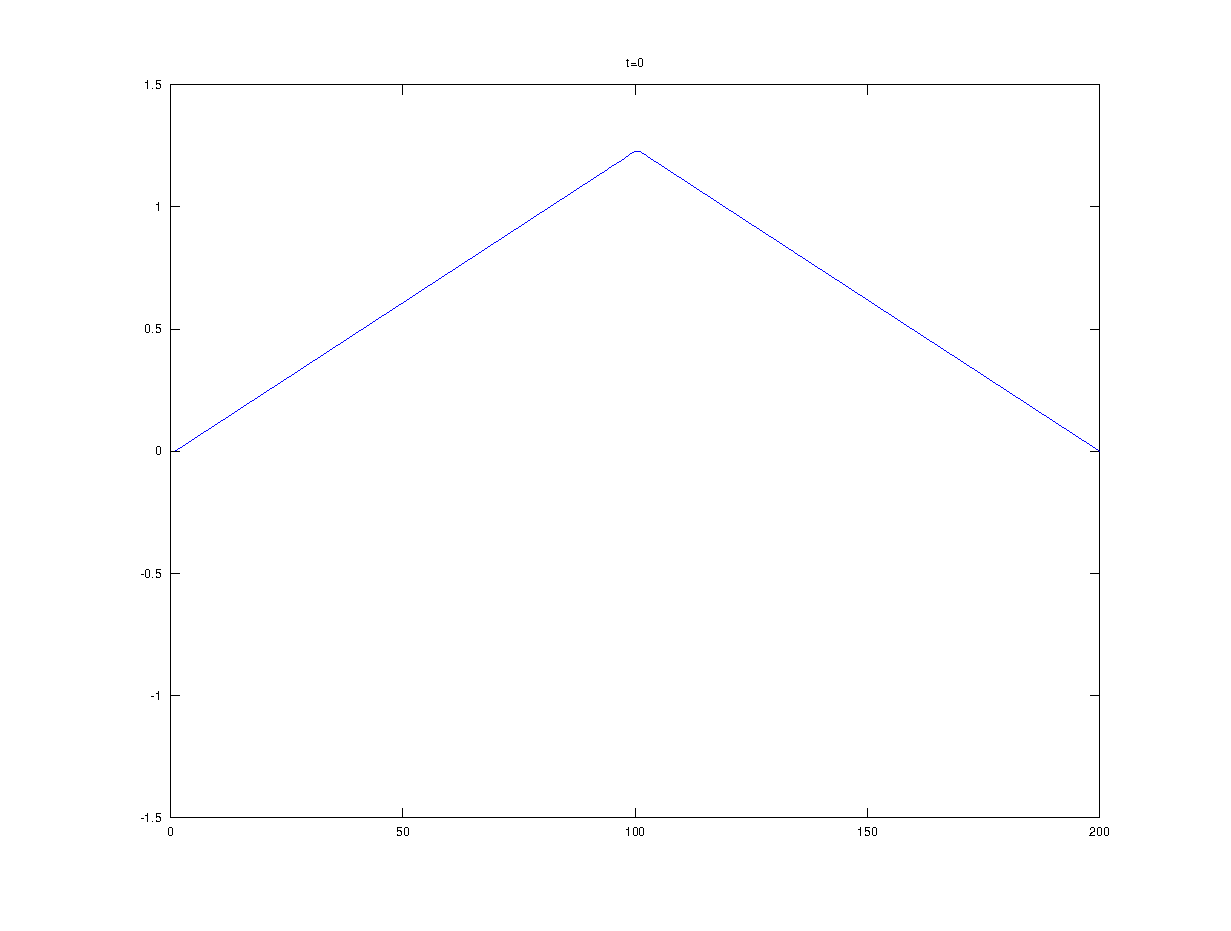
\includegraphics[width=6cm]{./fixed_ends_analytic_t0.eps}
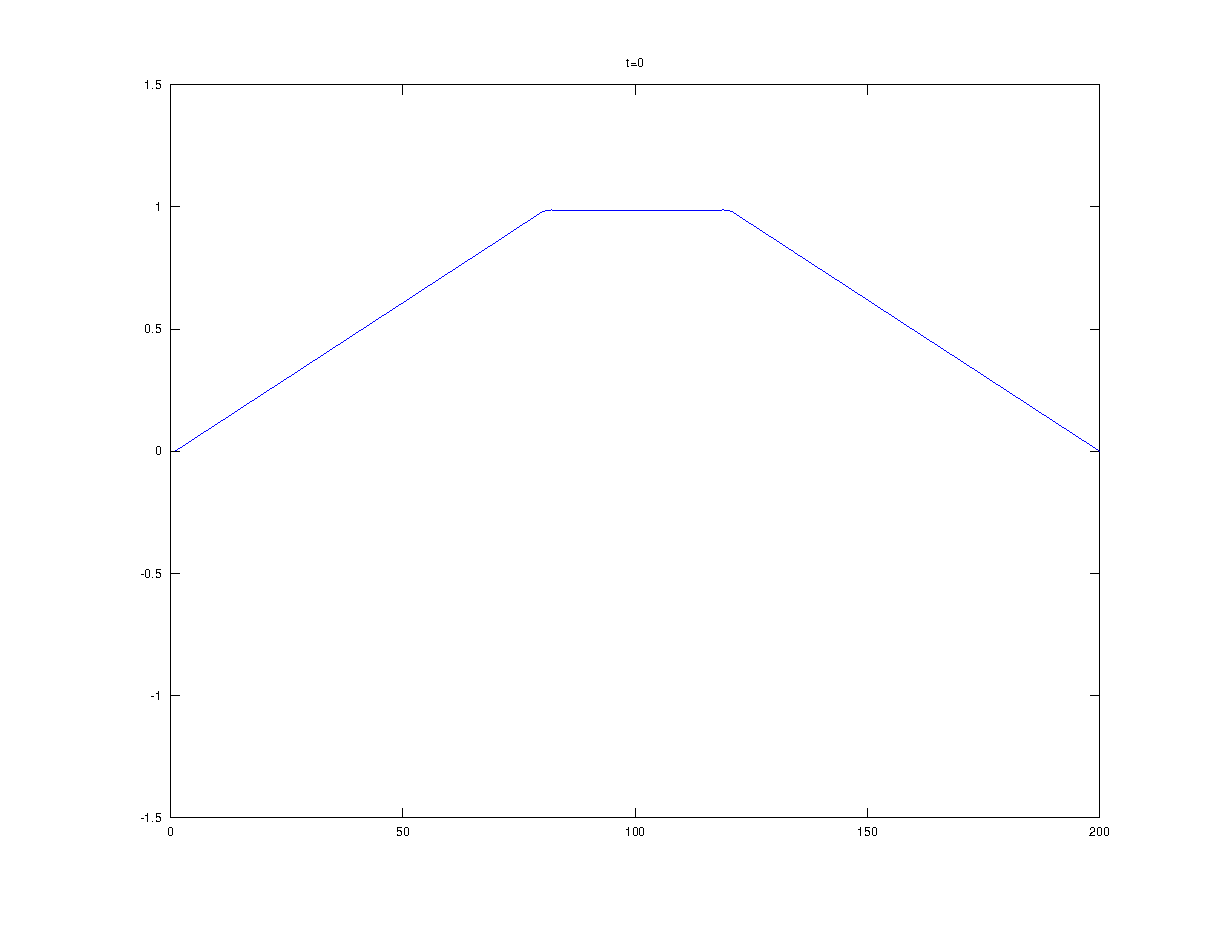
\includegraphics[width=6cm]{./fixed_ends_analytic_t0.1.eps}
 % fixed_ends_analytic.eps: 0x0 pixel, 300dpi, 0.00x0.00 cm, bb=
%\end{center}

\caption{Initial value problem, triangular shape, t=0 and 0.1}
\end{figure} 

\begin{figure}
%\begin{center}
 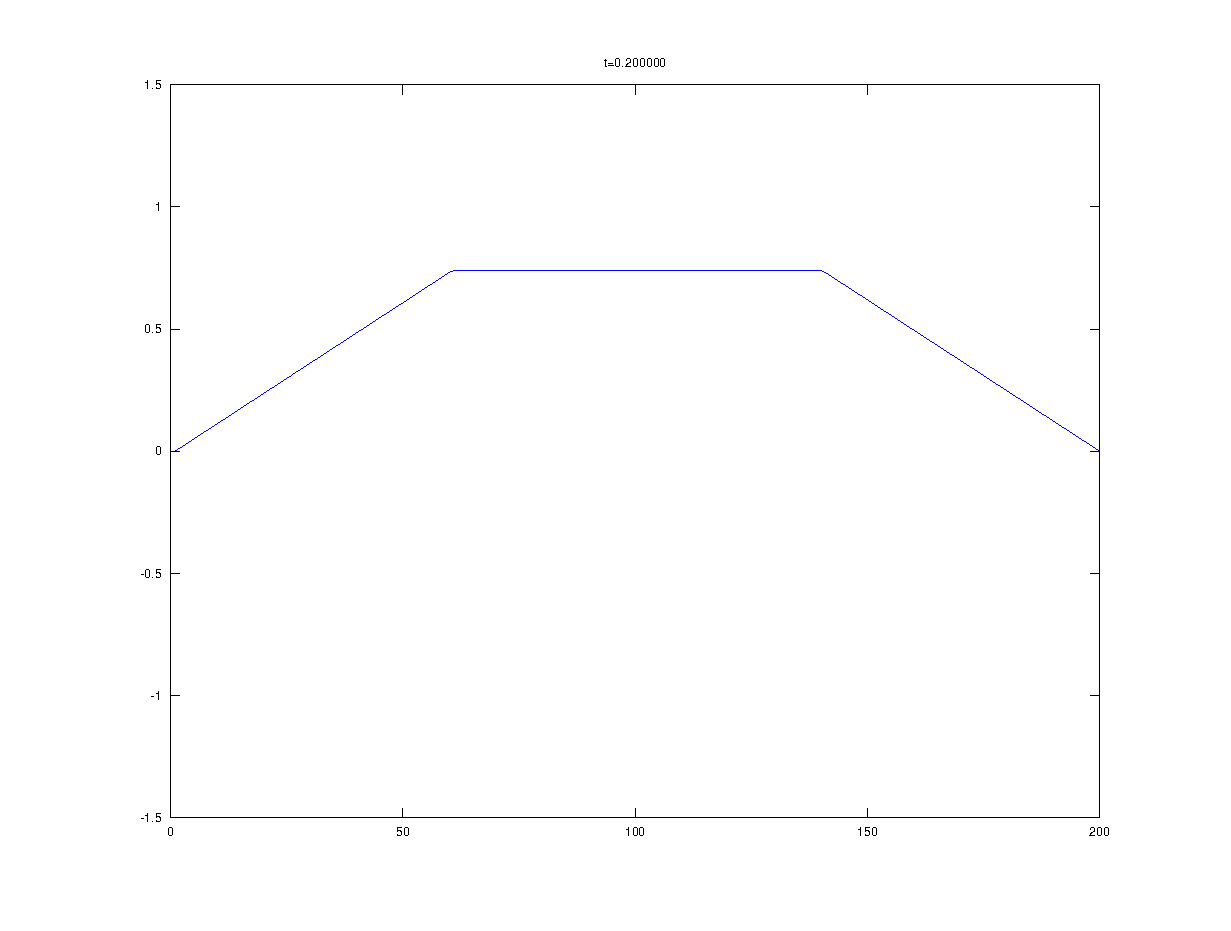
\includegraphics[width=6cm]{./fixed_ends_analytic_t0.200000.eps}
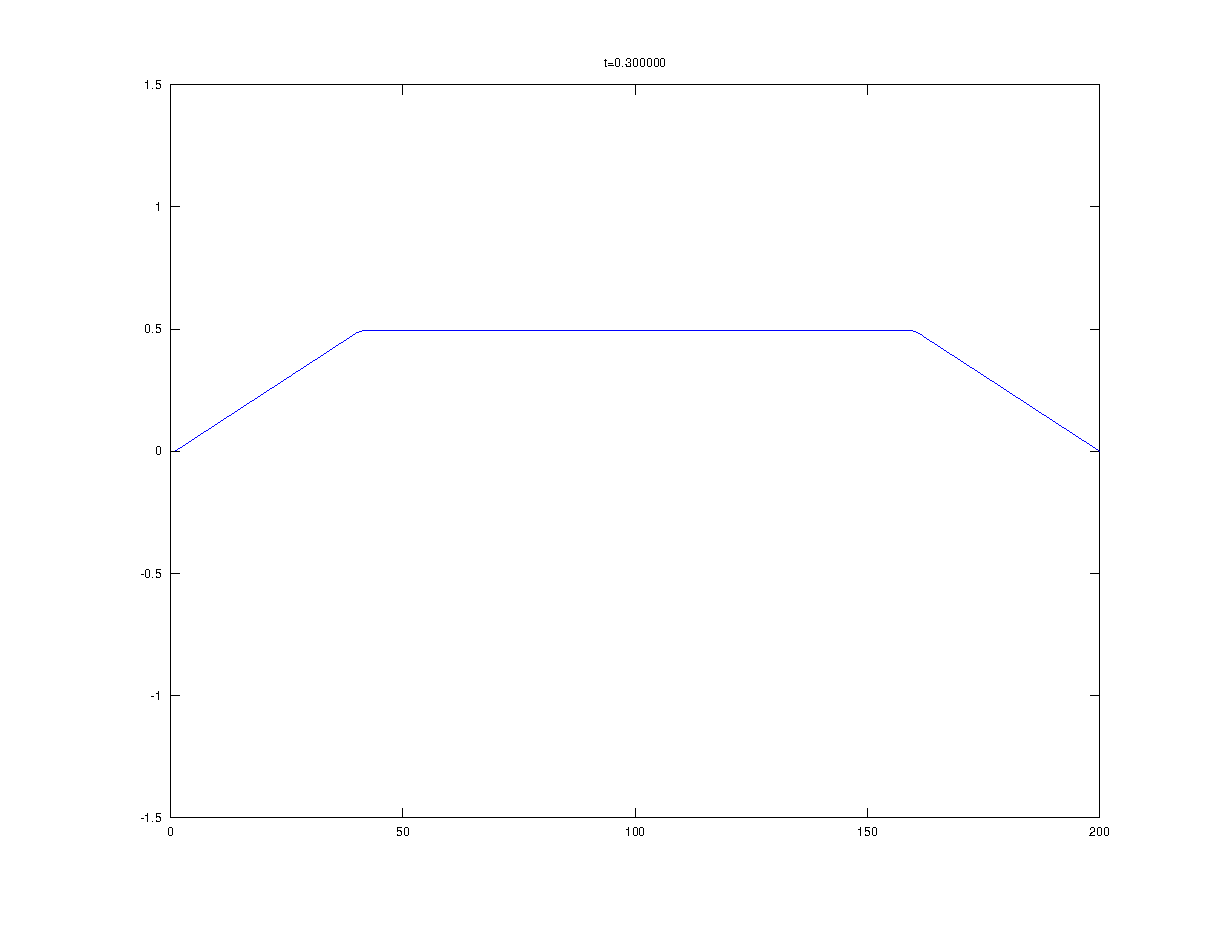
\includegraphics[width=6cm]{./fixed_ends_analytic_t0.300000.eps}
 % fixed_ends_analytic.eps: 0x0 pixel, 300dpi, 0.00x0.00 cm, bb=
%\end{center}

\caption{Initial value problem, triangular shape, t=0.2 and 0.3}
\end{figure} 

\begin{figure}
%\begin{center}
 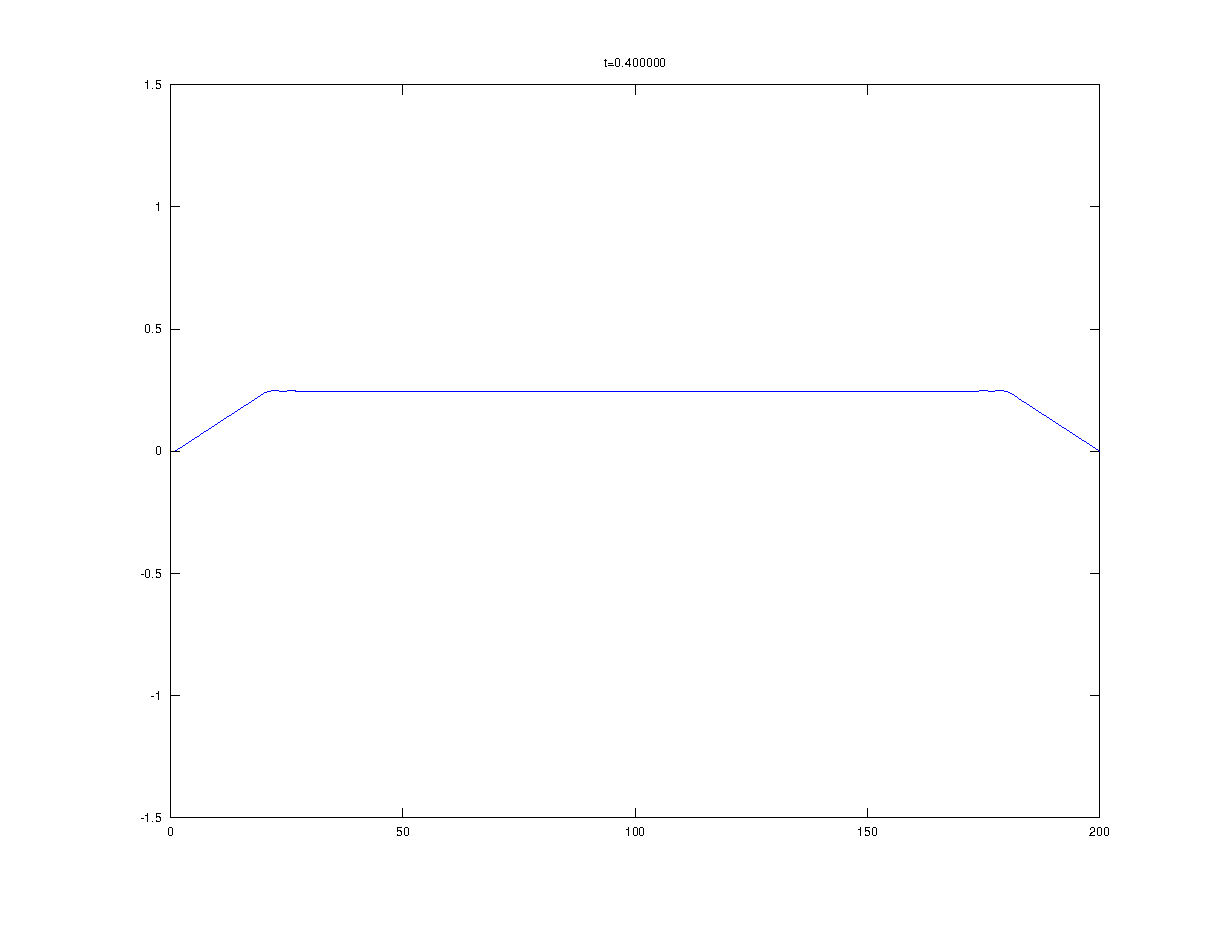
\includegraphics[width=6cm]{./fixed_ends_analytic_t0.400000.eps}
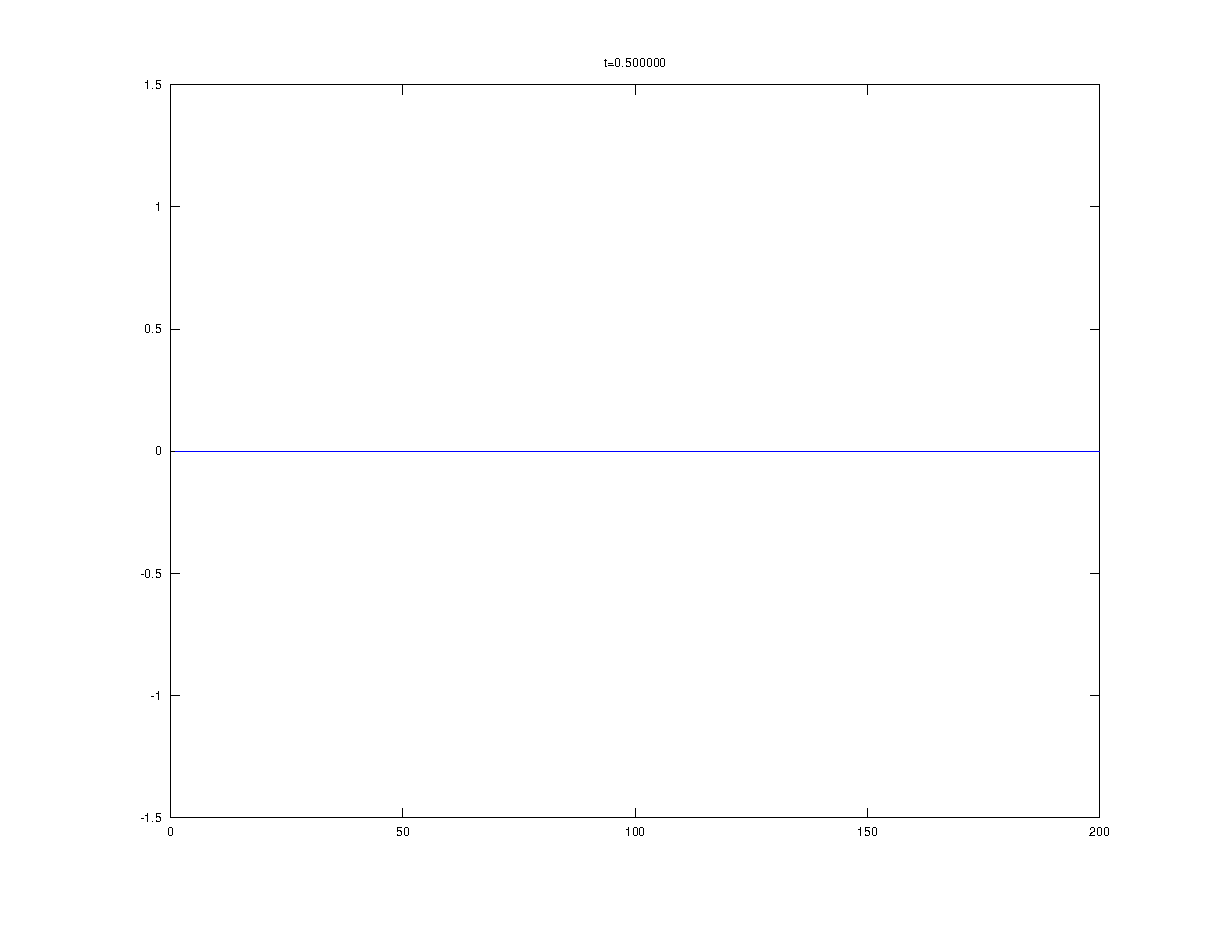
\includegraphics[width=6cm]{./fixed_ends_analytic_t0.500000.eps}
 % fixed_ends_analytic.eps: 0x0 pixel, 300dpi, 0.00x0.00 cm, bb=
%\end{center}

\caption{Initial value problem, triangular shape, t=0.4 and 0.5}
\end{figure}
 
\begin{figure}
%\begin{center}
 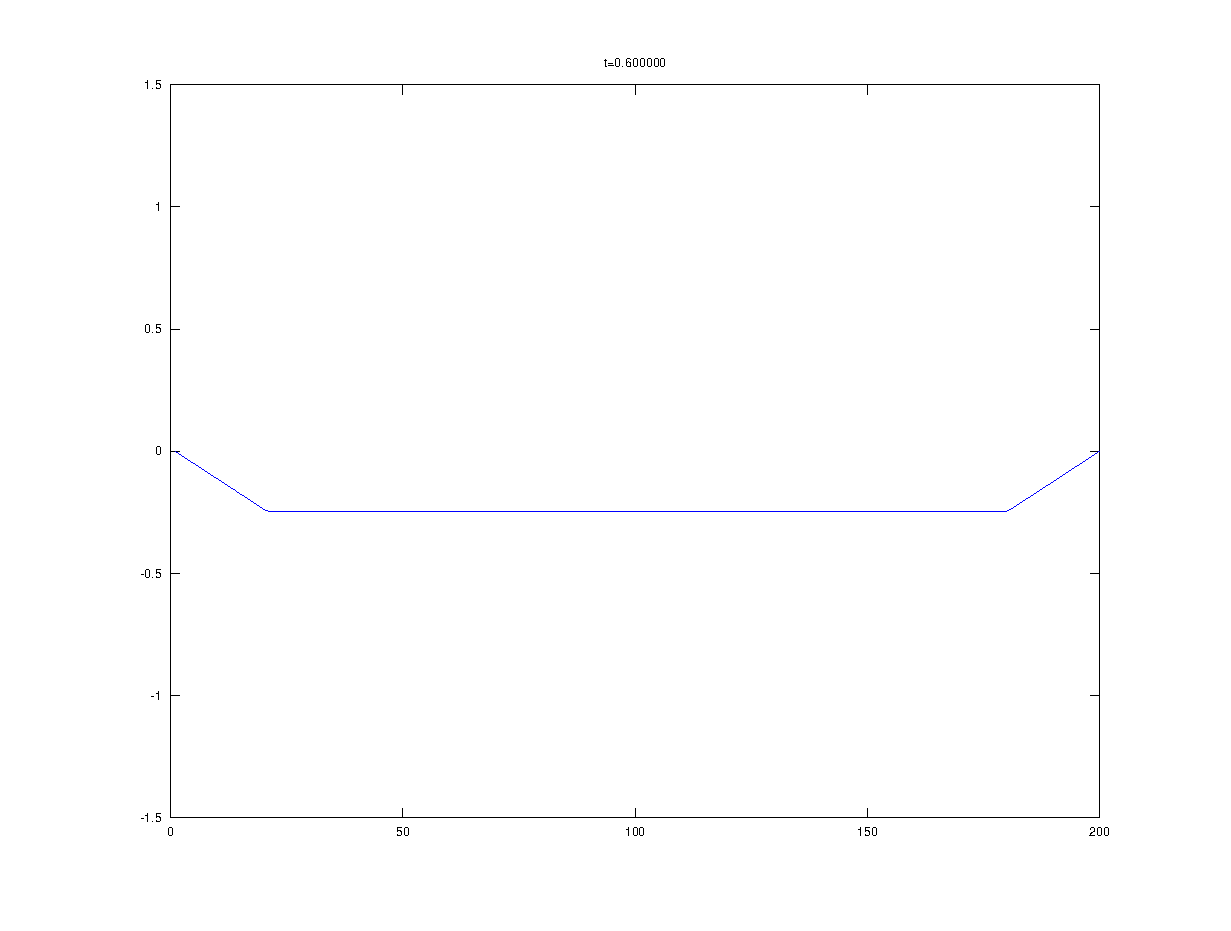
\includegraphics[width=6cm]{./fixed_ends_analytic_t0.600000.eps}
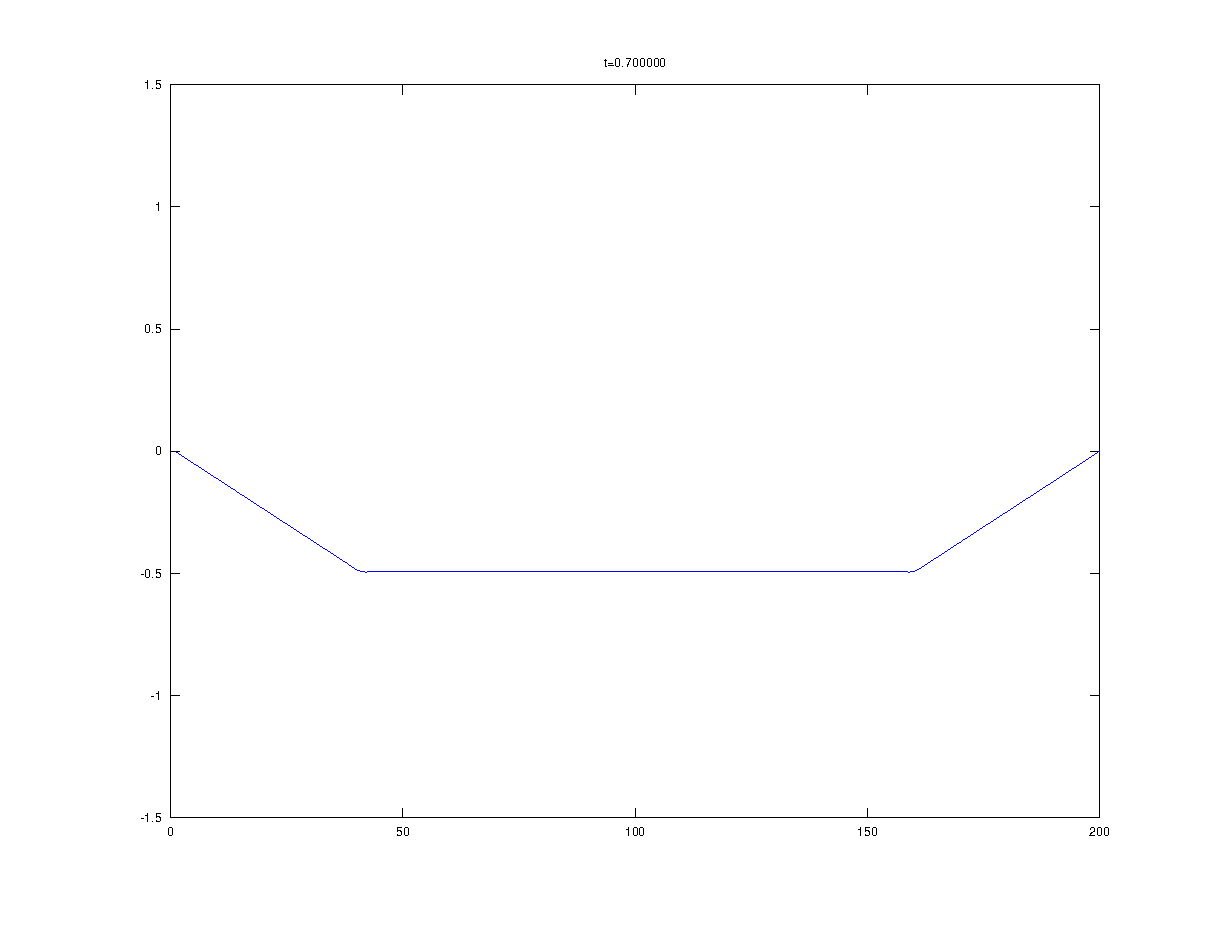
\includegraphics[width=6cm]{./fixed_ends_analytic_t0.700000.eps}
 % fixed_ends_analytic.eps: 0x0 pixel, 300dpi, 0.00x0.00 cm, bb=
%\end{center}

\caption{Initial value problem, triangular shape, t=0.6 and 0.7}
\end{figure} 

\begin{figure}
%\begin{center}
 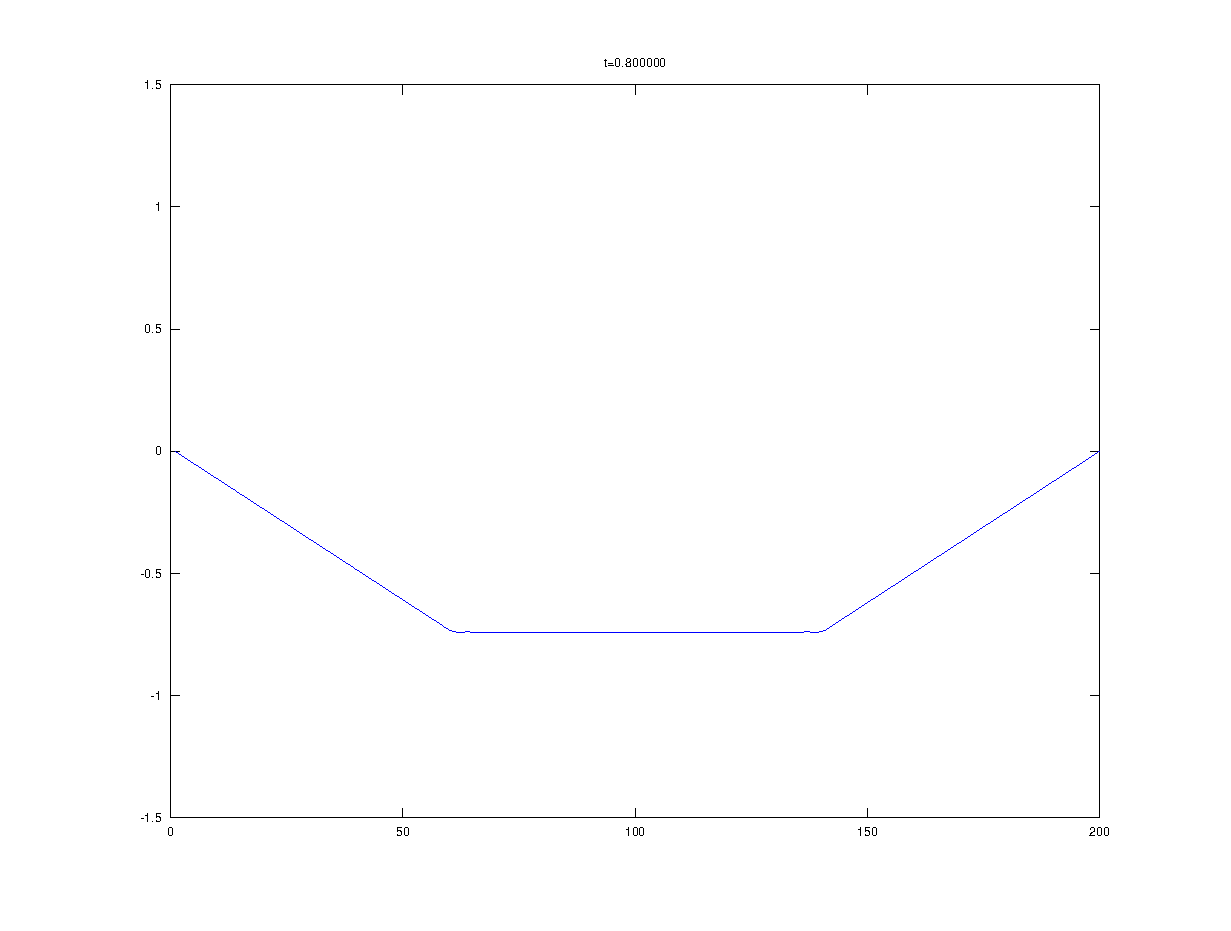
\includegraphics[width=6cm]{./fixed_ends_analytic_t0.800000.eps}
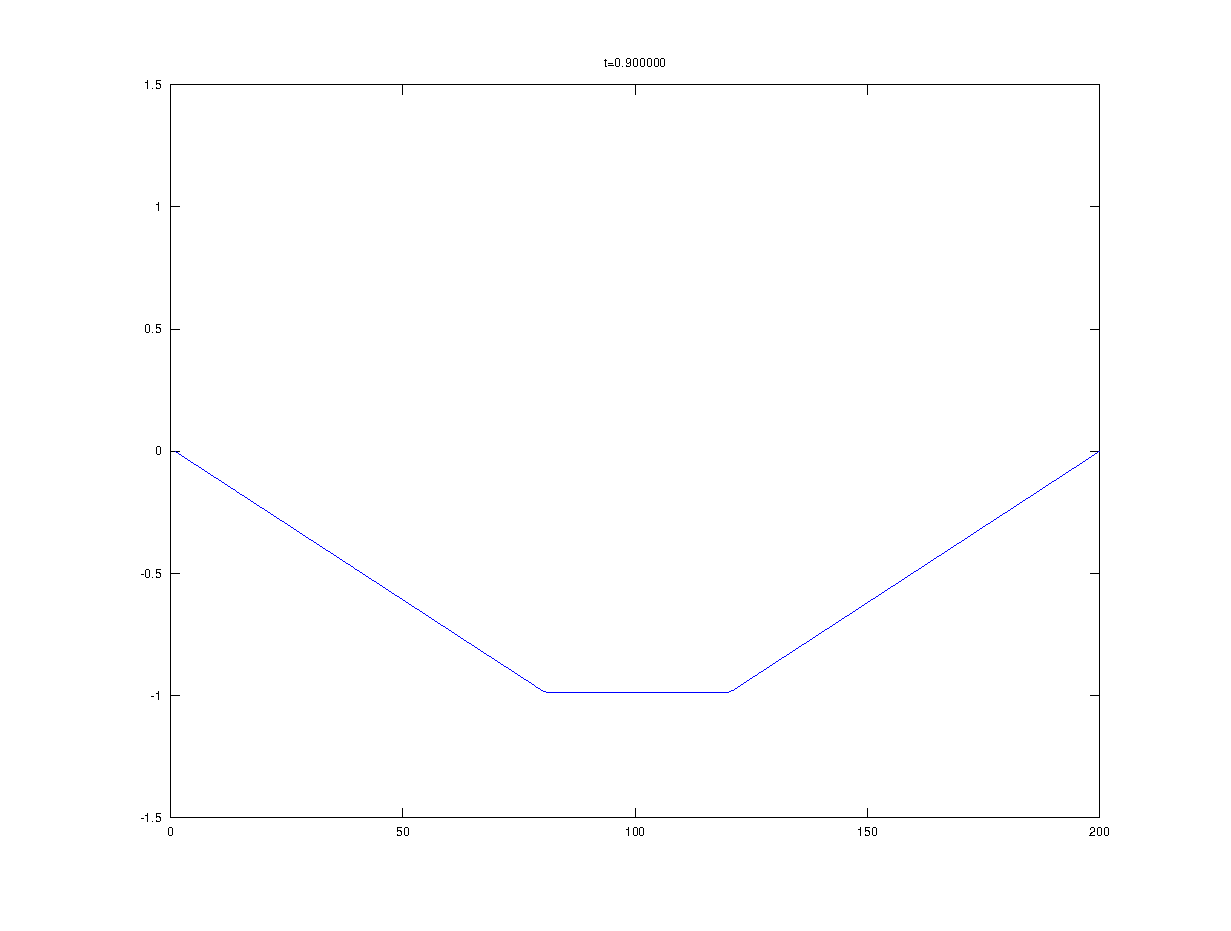
\includegraphics[width=6cm]{./fixed_ends_analytic_t0.900000.eps}
 % fixed_ends_analytic.eps: 0x0 pixel, 300dpi, 0.00x0.00 cm, bb=
%\end{center}

\caption{Initial value problem, triangular shape, t=0.8 and 0.9}
\end{figure} 

\begin{figure}
%\begin{center}
 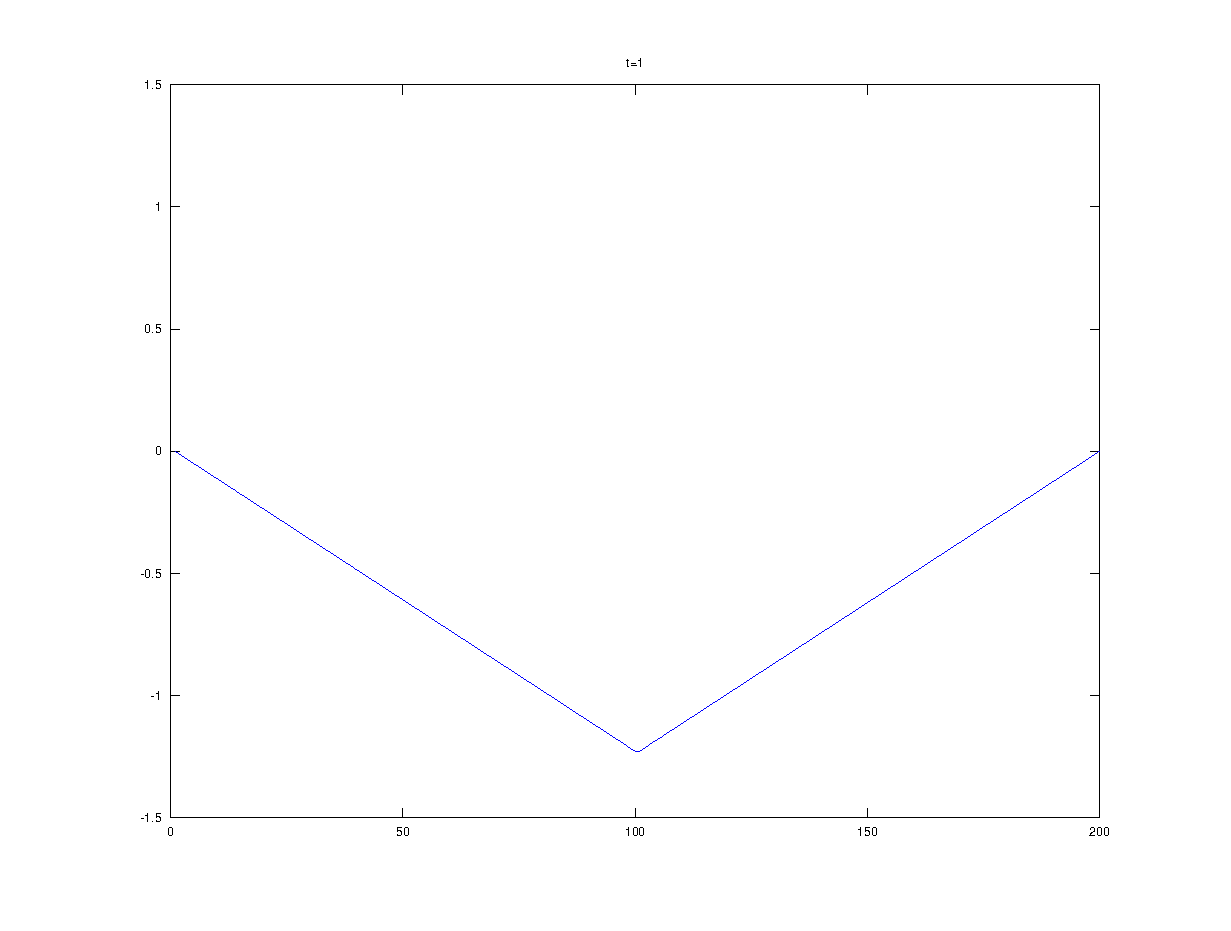
\includegraphics[width=6cm]{./fixed_ends_analytic_t1.eps}
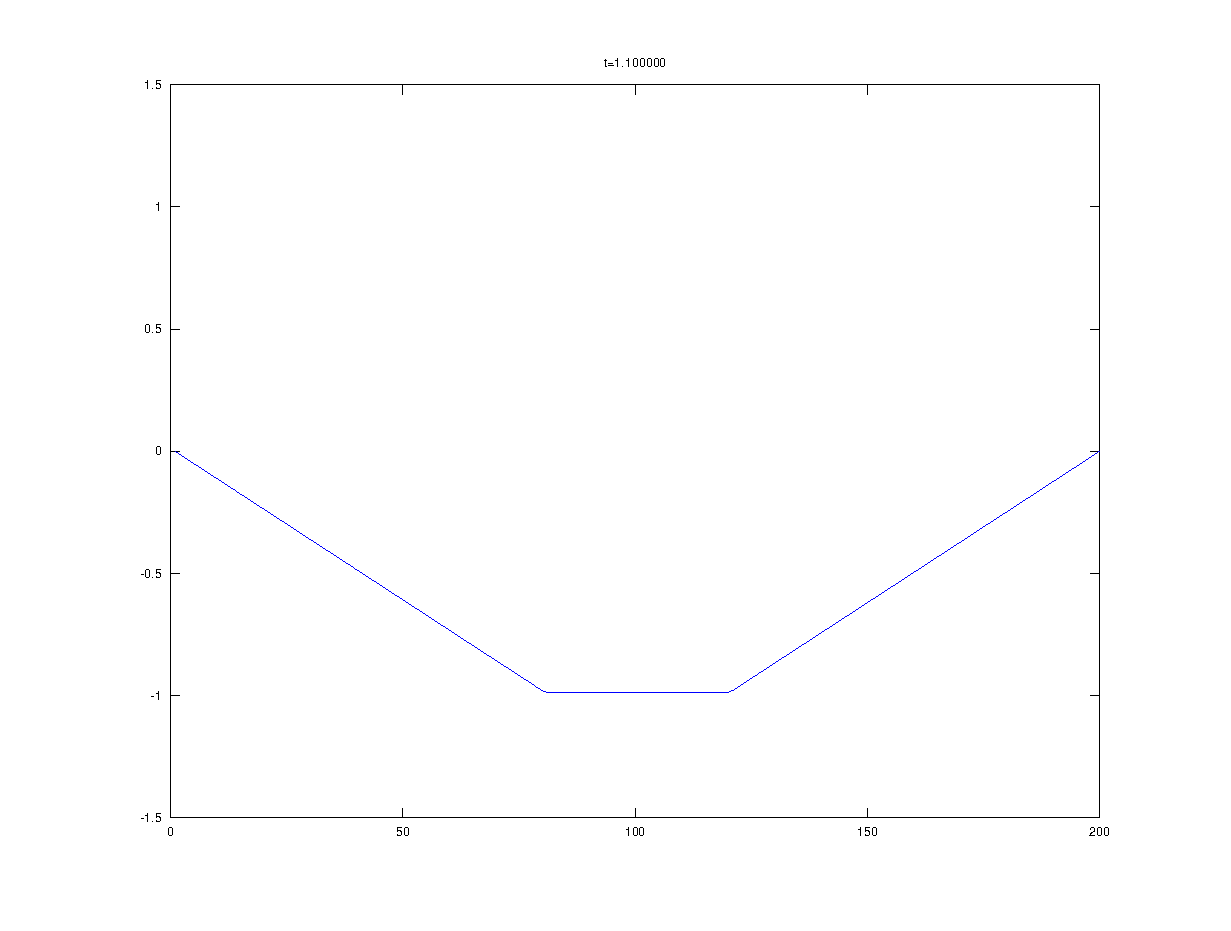
\includegraphics[width=6cm]{./fixed_ends_analytic_t1.100000.eps}
 % fixed_ends_analytic.eps: 0x0 pixel, 300dpi, 0.00x0.00 cm, bb=
%\end{center}

\caption{Initial value problem, triangular shape, t=1.0 and 1.1}
\end{figure} 

\begin{figure}
%\begin{center}
 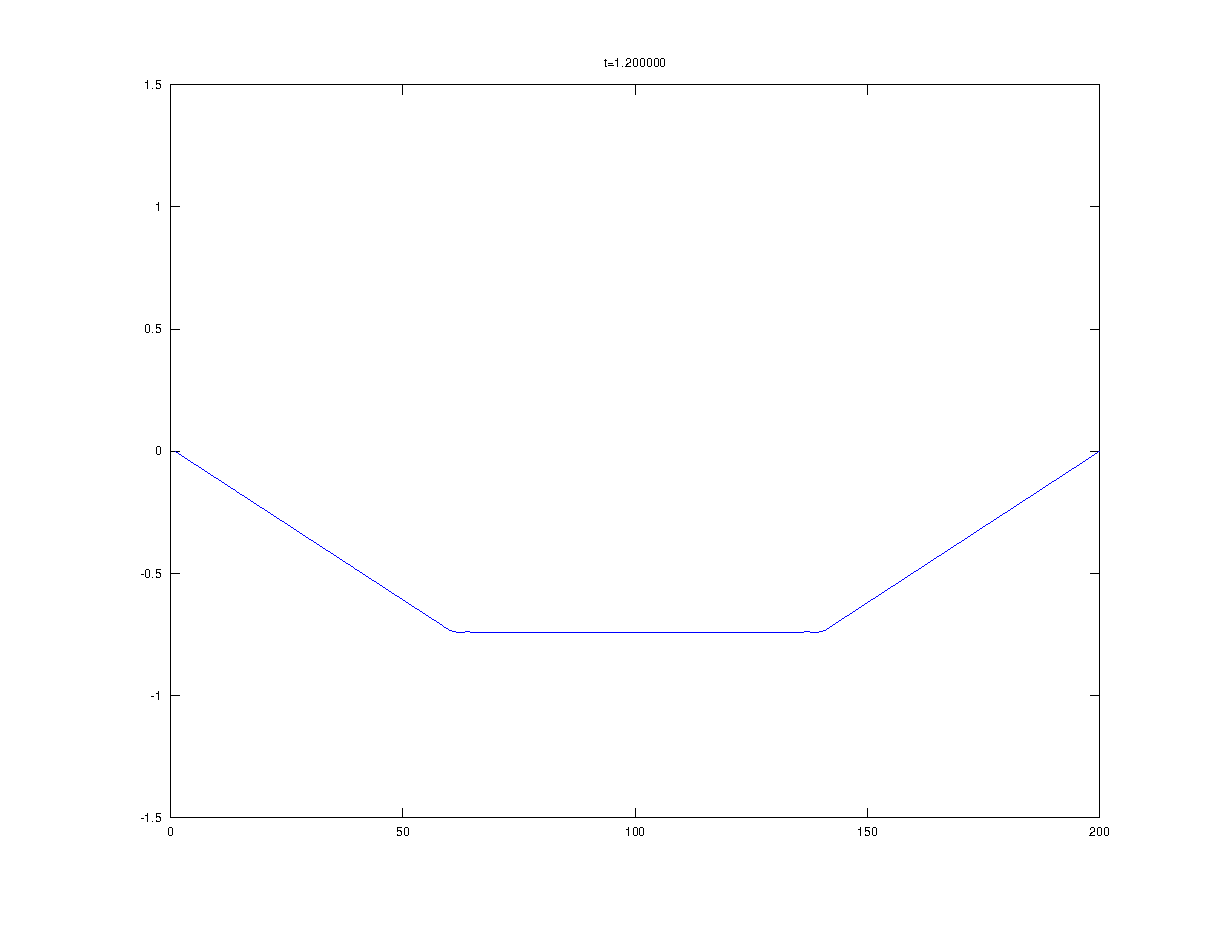
\includegraphics[width=6cm]{./fixed_ends_analytic_t1.200000.eps}
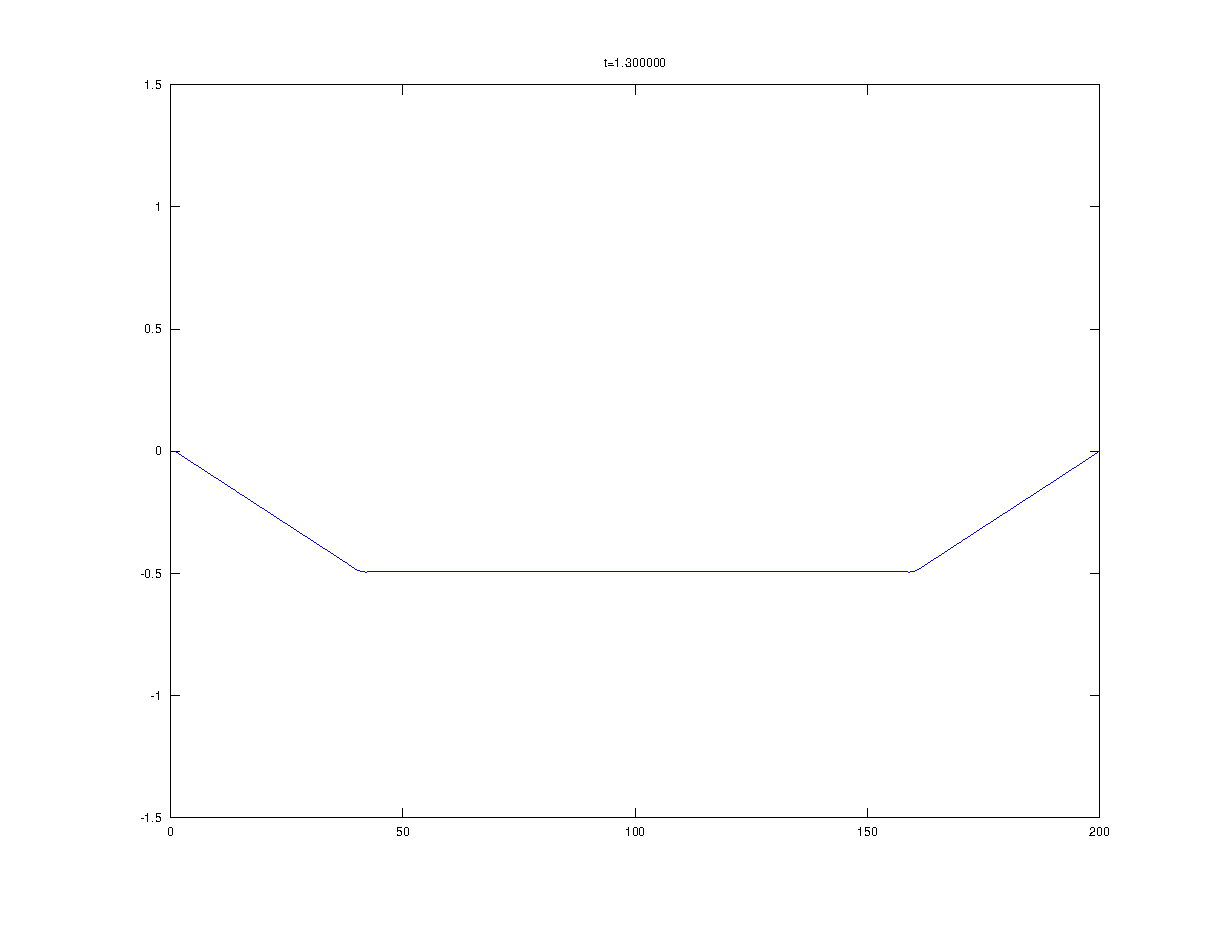
\includegraphics[width=6cm]{./fixed_ends_analytic_t1.300000.eps}
 % fixed_ends_analytic.eps: 0x0 pixel, 300dpi, 0.00x0.00 cm, bb=
%\end{center}

\caption{Initial value problem, triangular shape, t=1.2 and 1.3}
\end{figure} 

\begin{figure}
%\begin{center}
 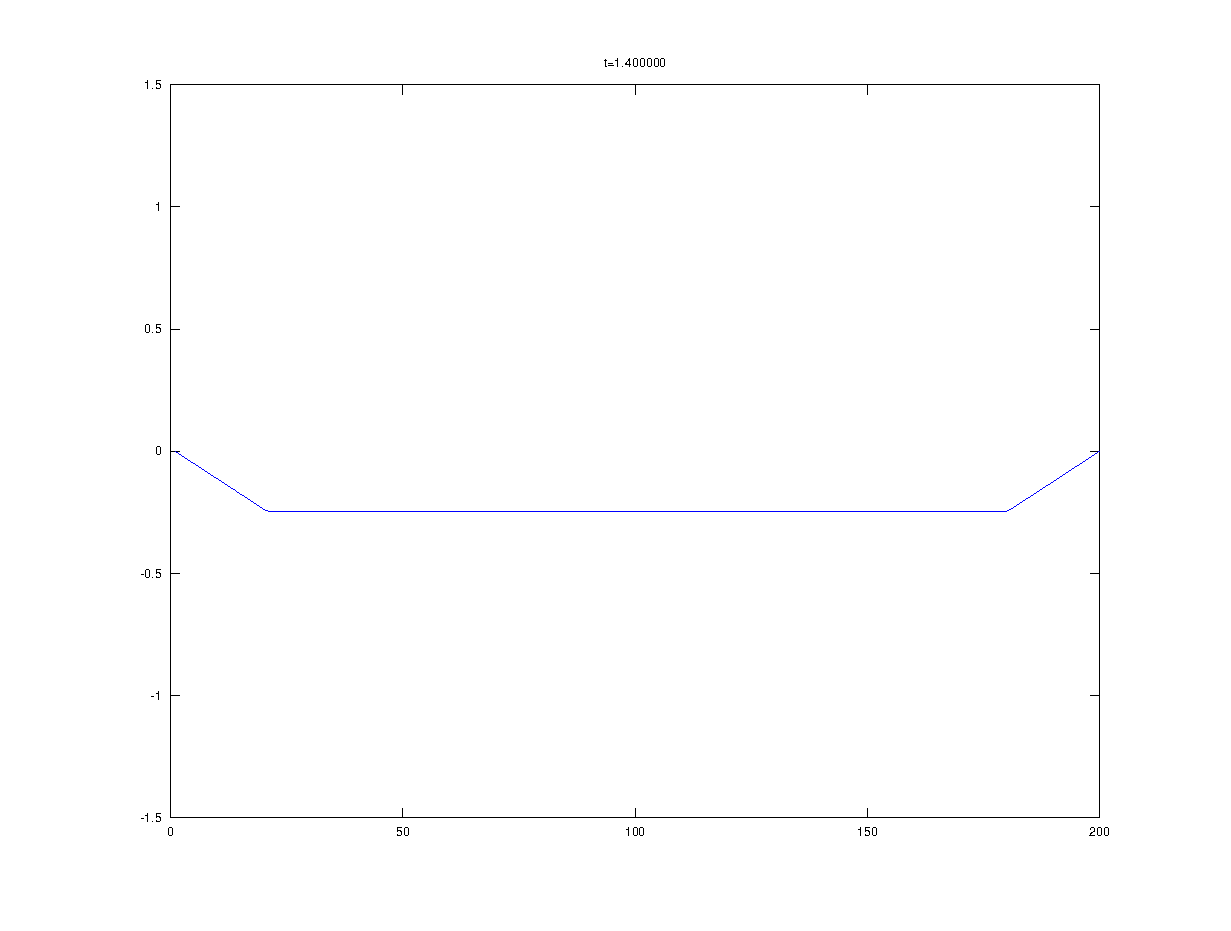
\includegraphics[width=6cm]{./fixed_ends_analytic_t1.400000.eps}
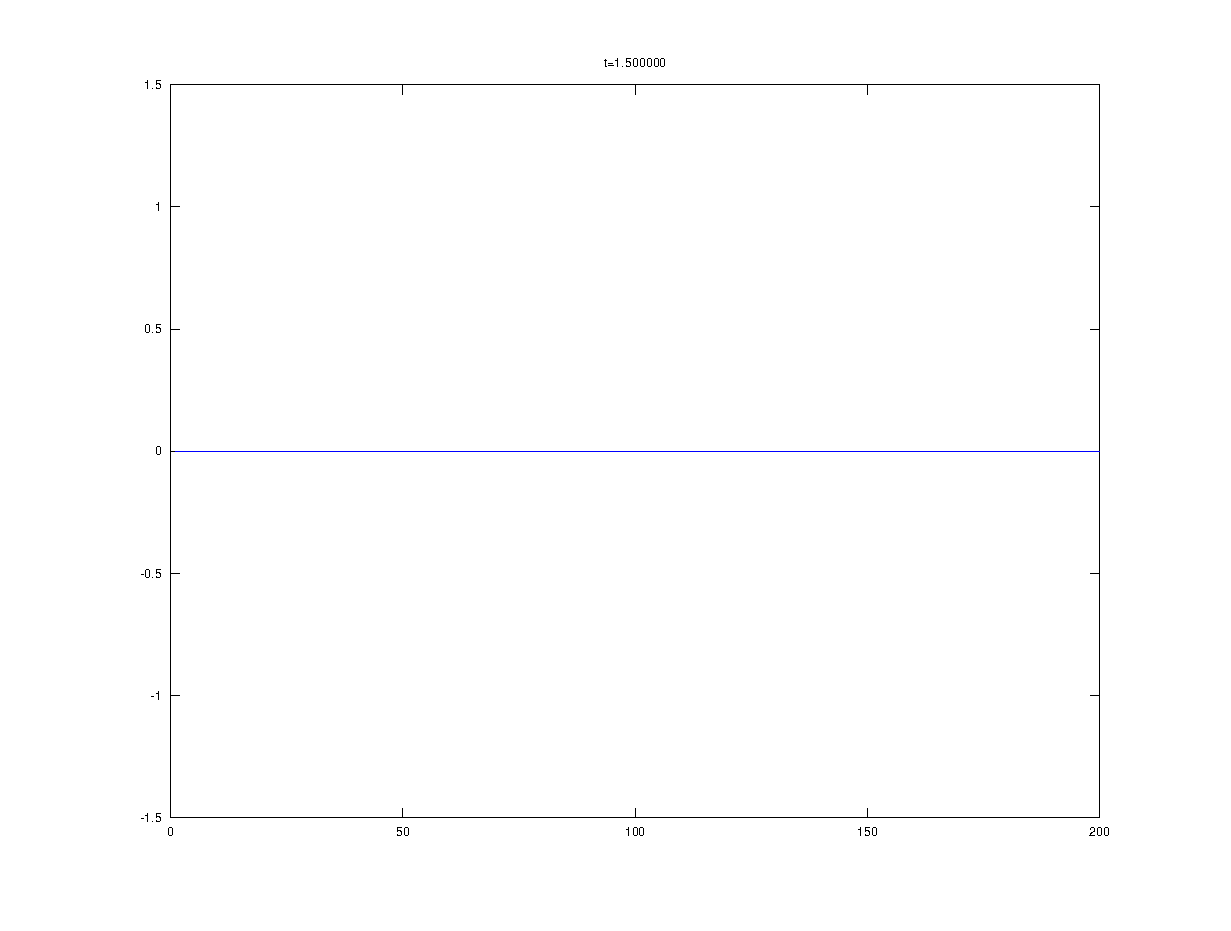
\includegraphics[width=6cm]{./fixed_ends_analytic_t1.500000.eps}
 % fixed_ends_analytic.eps: 0x0 pixel, 300dpi, 0.00x0.00 cm, bb=
%\end{center}

\caption{Initial value problem, triangular shape, t=0.4 and 0.5}
\end{figure} 

\begin{figure}
%\begin{center}
 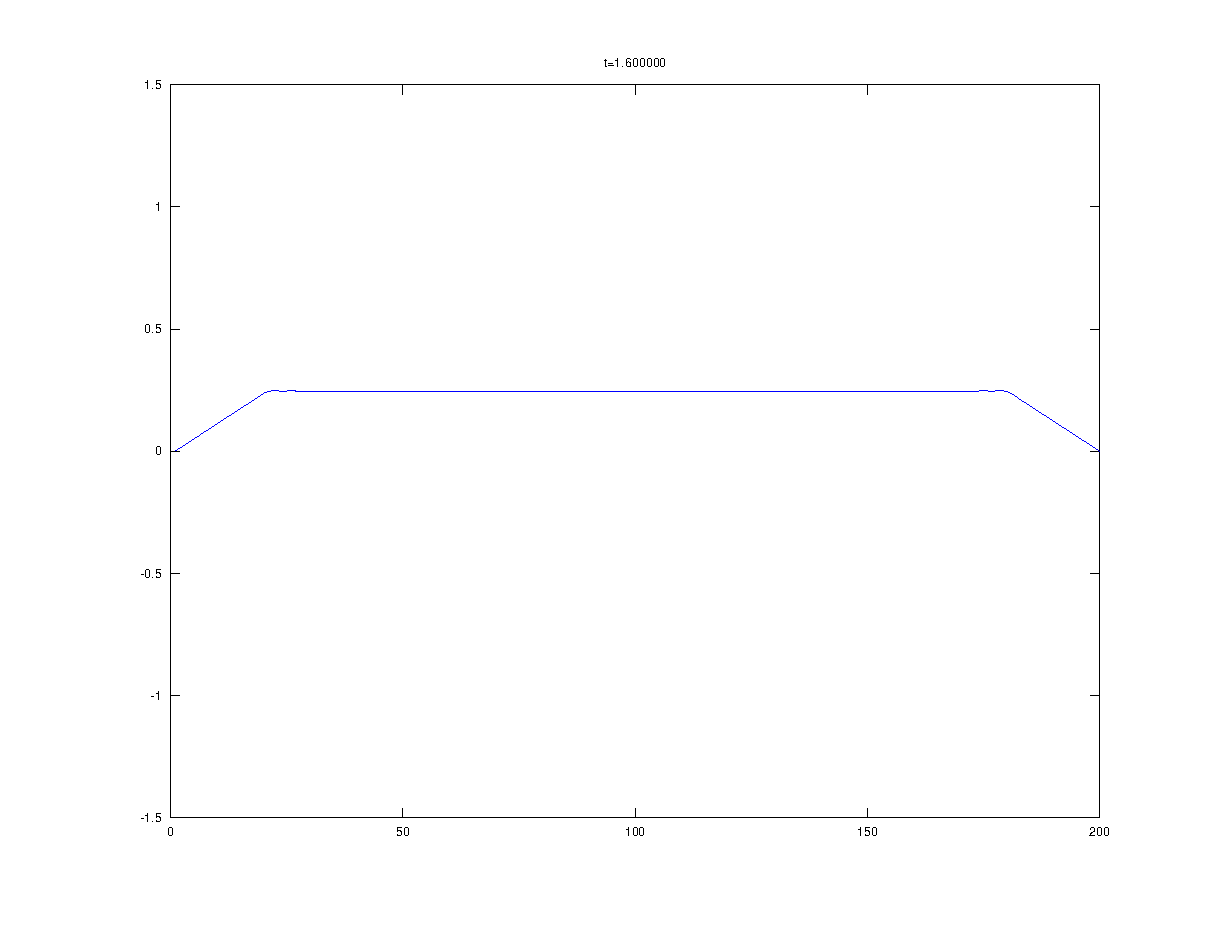
\includegraphics[width=6cm]{./fixed_ends_analytic_t1.600000.eps}
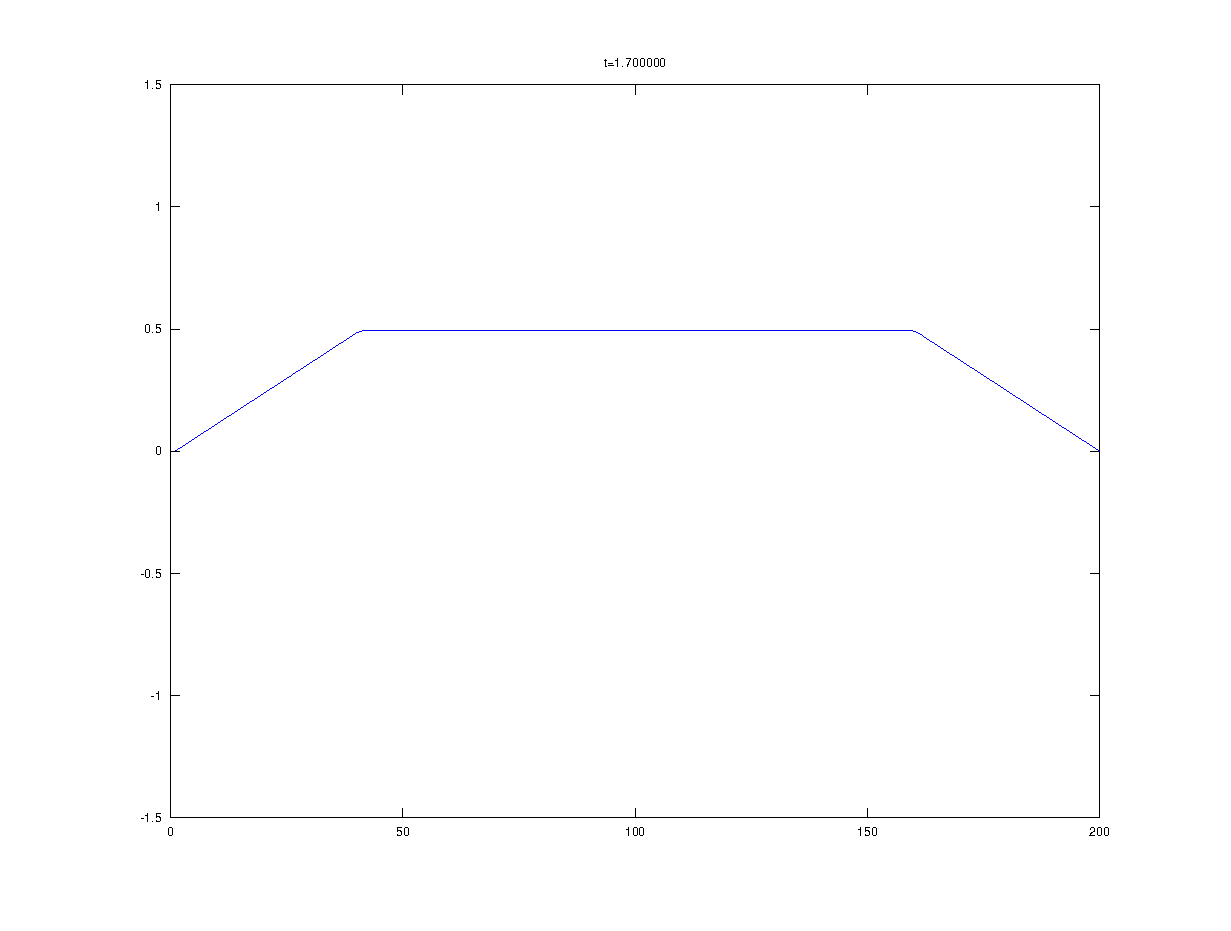
\includegraphics[width=6cm]{./fixed_ends_analytic_t1.700000.eps}
 % fixed_ends_analytic.eps: 0x0 pixel, 300dpi, 0.00x0.00 cm, bb=
%\end{center}

\caption{Initial value problem, triangular shape, t=1.6 and 1.7}
\end{figure} 

\begin{figure}
%\begin{center}
 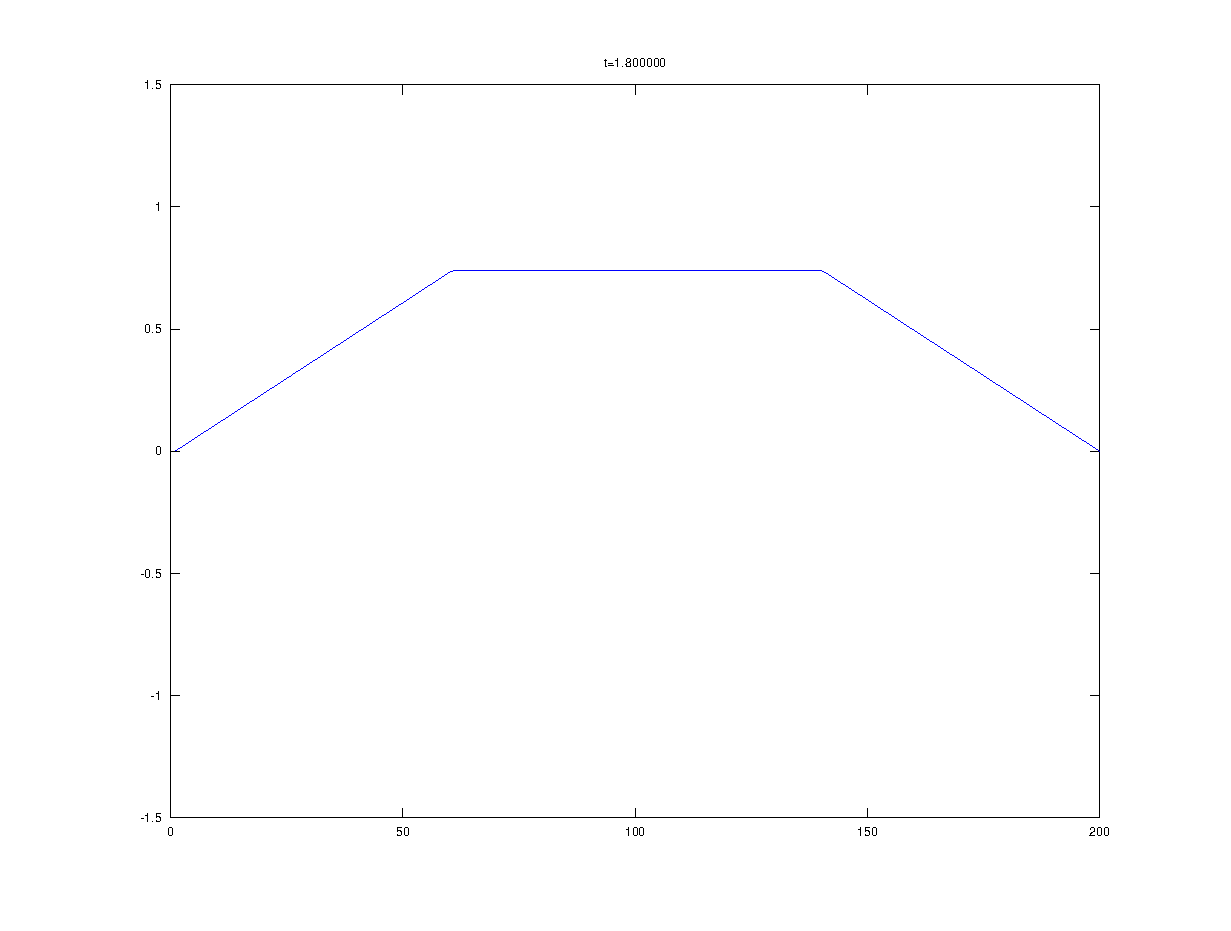
\includegraphics[width=6cm]{./fixed_ends_analytic_t1.800000.eps}
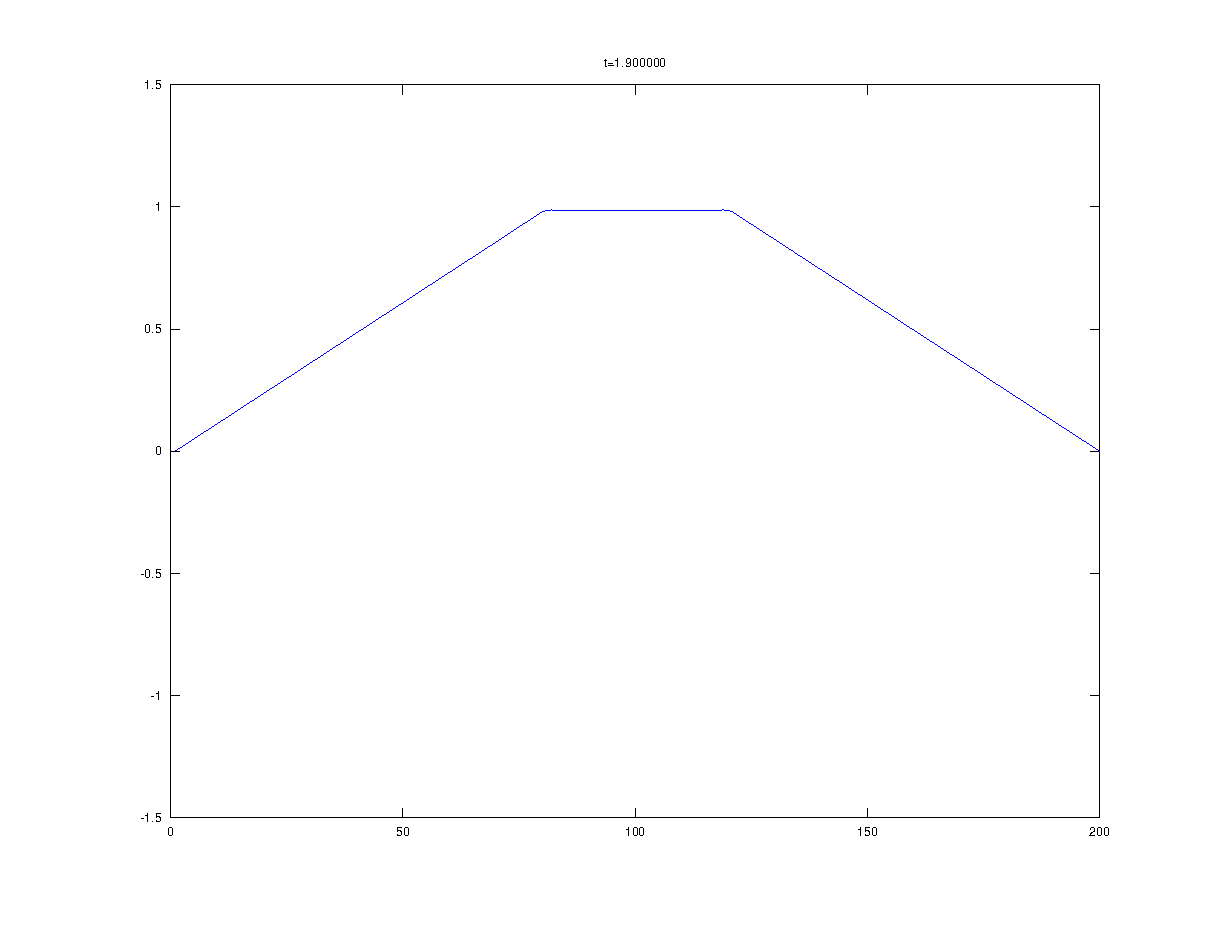
\includegraphics[width=6cm]{./fixed_ends_analytic_t1.900000.eps}
 % fixed_ends_analytic.eps: 0x0 pixel, 300dpi, 0.00x0.00 cm, bb=
%\end{center}

\caption{Initial value problem, triangular shape, t=0.8 and 0.9}
\label{fig:bounded_2}
\end{figure} 

\section{String, fixed on one end}
In this test configuration, a string with wavespeed one is fixed on one end and loose on the other. The inithial shape corresponds to a cosine function and the initial speed is zero. 
The results are presented in Figures \ref{fig:half_bounded_1} to \ref{fig:half_bounded_2}. 

\begin{figure}
%\begin{center}
 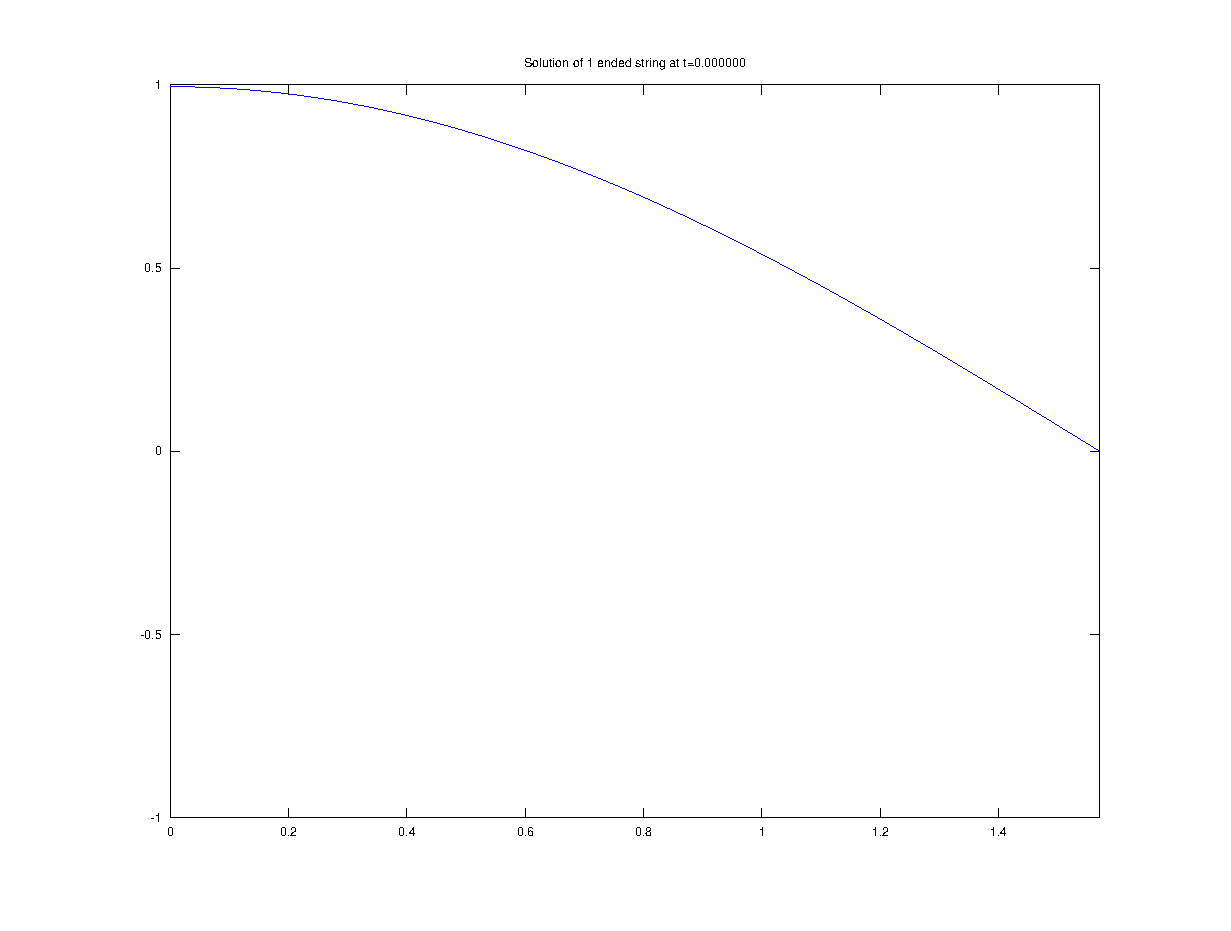
\includegraphics[width=6cm]{./one_fixed_end_analytic_t0.000000.eps}
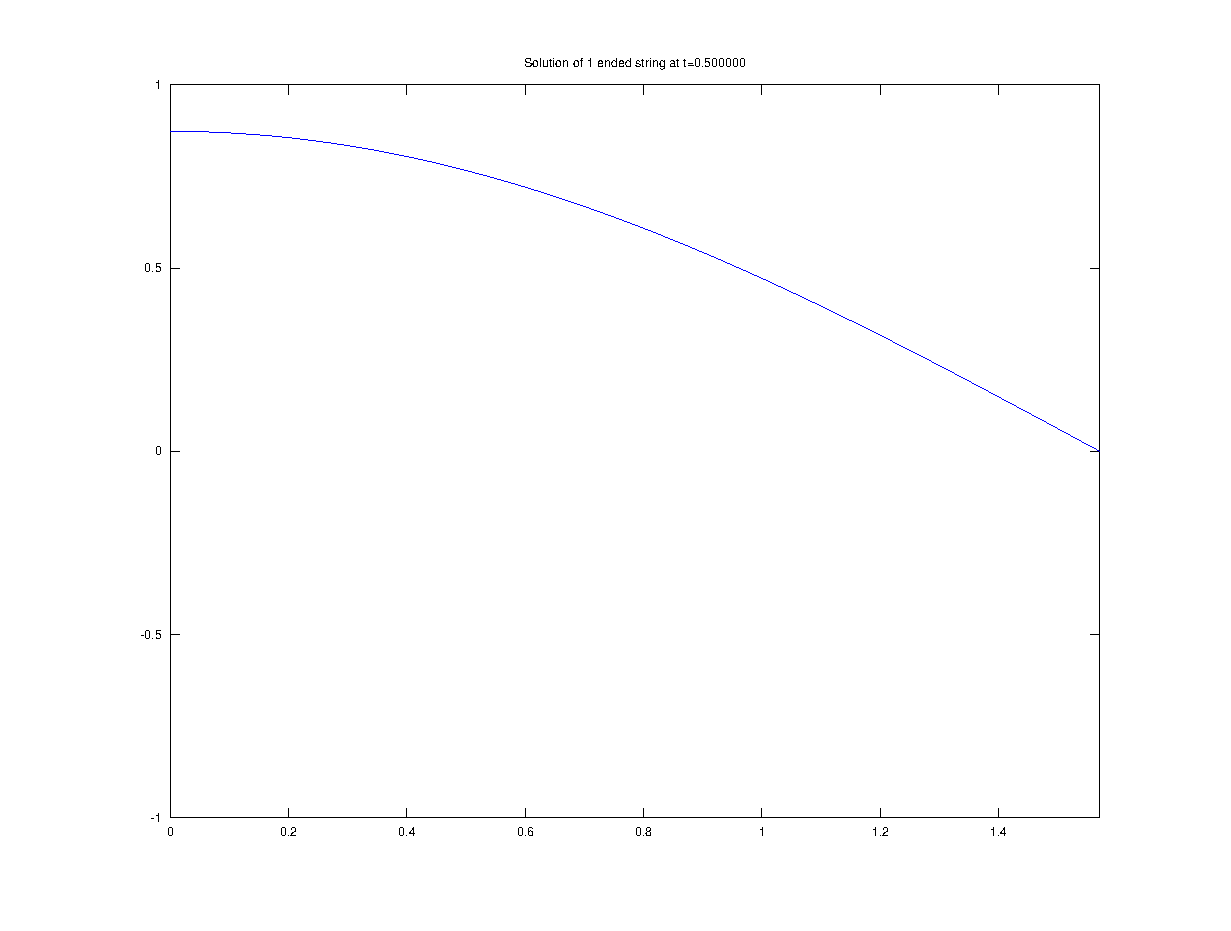
\includegraphics[width=6cm]{./one_fixed_end_analytic_t0.500000.eps}
 % fixed_ends_analytic.eps: 0x0 pixel, 300dpi, 0.00x0.00 cm, bb=
%\end{center}

\caption{Initial value problem, a string fixed on one end, t=0 and 0.5}
\label{fig:half_bounded_1}
\end{figure} 

\begin{figure}
%\begin{center}
 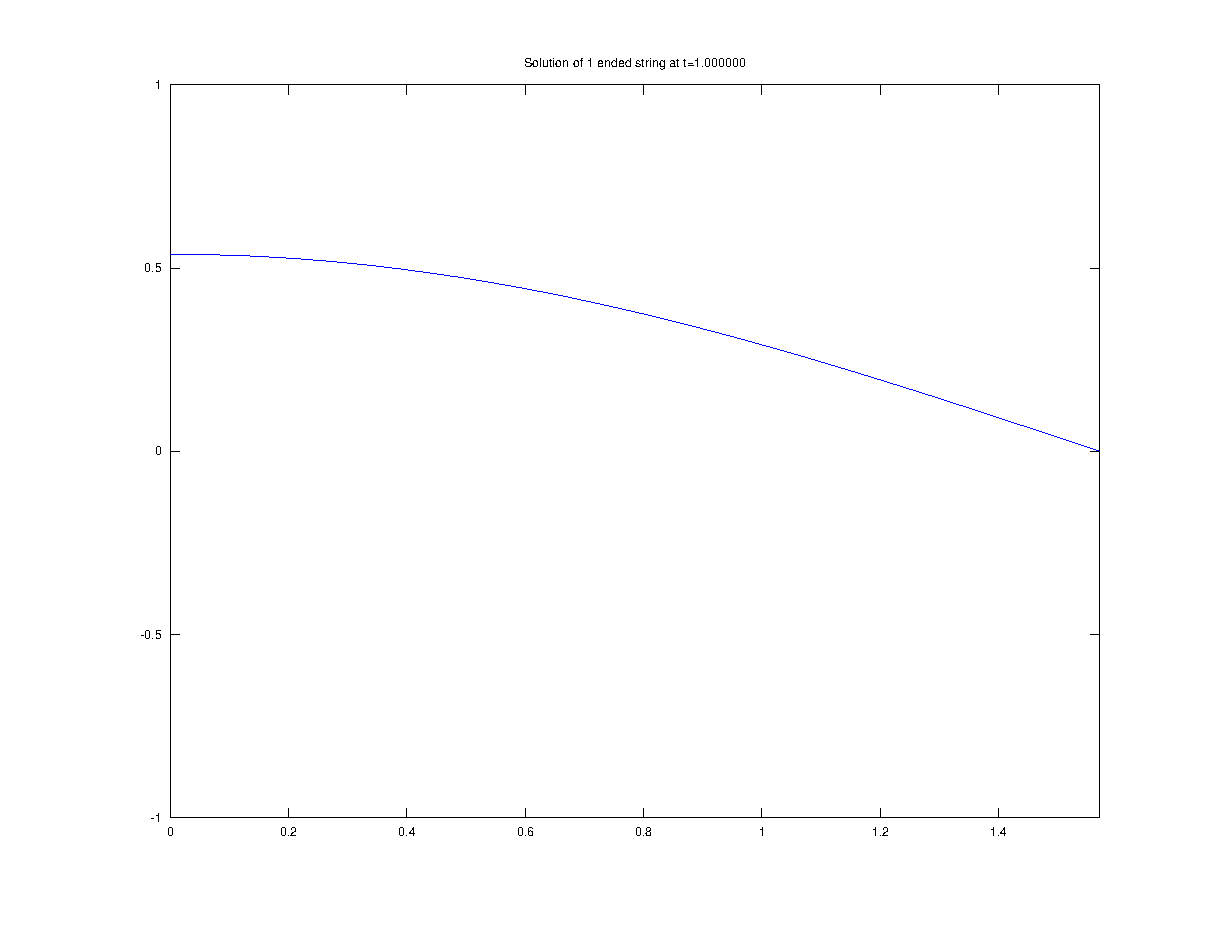
\includegraphics[width=6cm]{./one_fixed_end_analytic_t1.000000.eps}
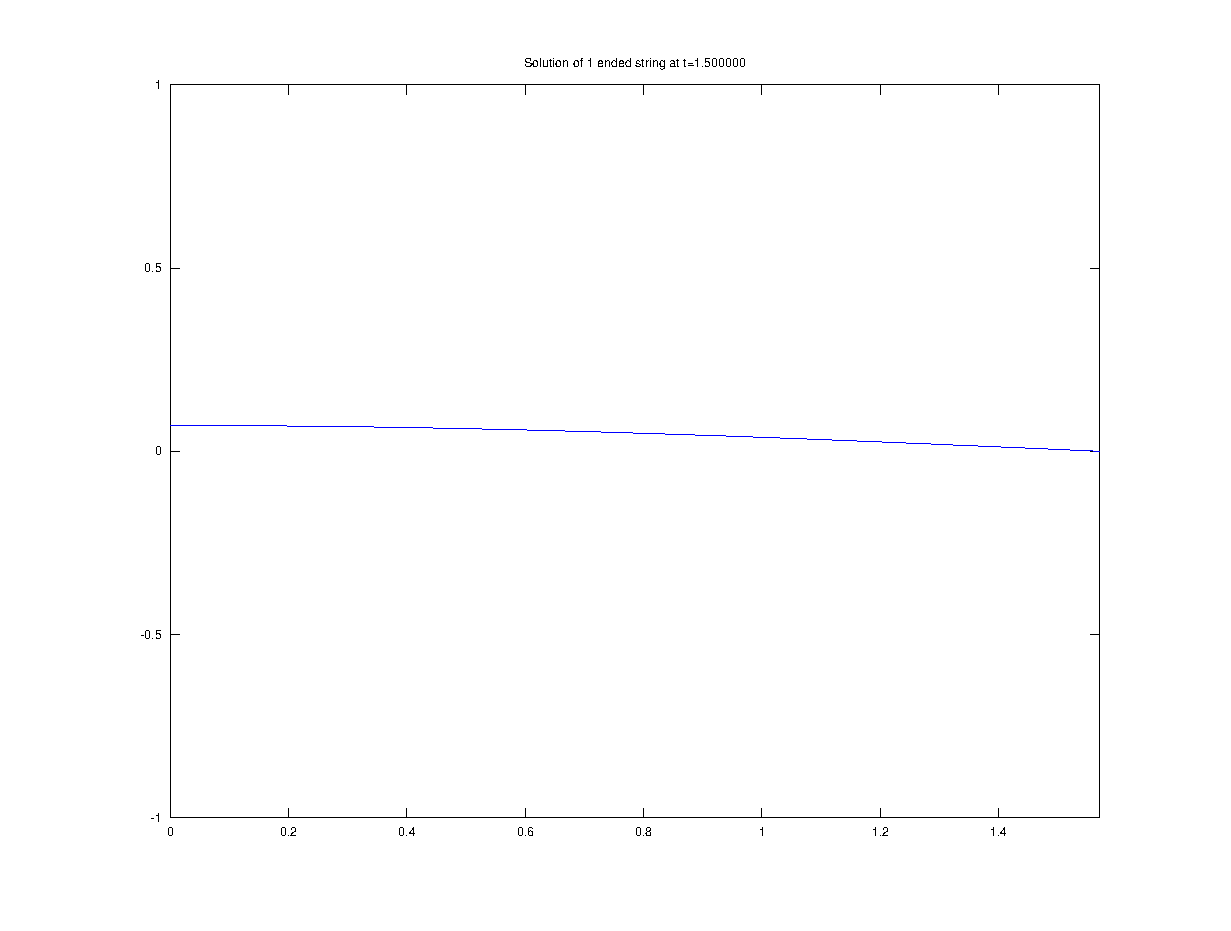
\includegraphics[width=6cm]{./one_fixed_end_analytic_t1.500000.eps}
 % fixed_ends_analytic.eps: 0x0 pixel, 300dpi, 0.00x0.00 cm, bb=
%\end{center}

\caption{Initial value problem, a string fixed on one end, t=1 and 1.5}

\end{figure} 

\begin{figure}
%\begin{center}
 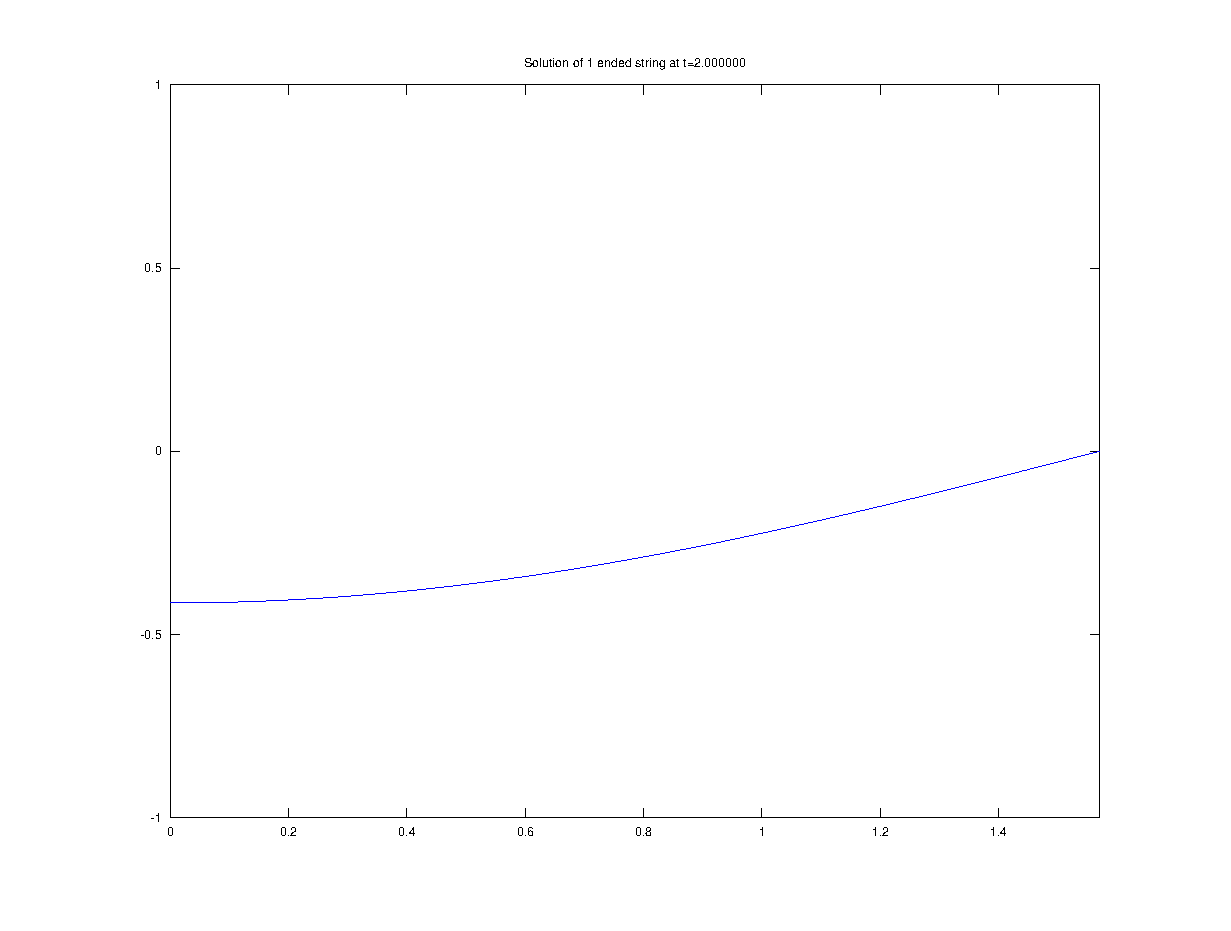
\includegraphics[width=6cm]{./one_fixed_end_analytic_t2.000000.eps}
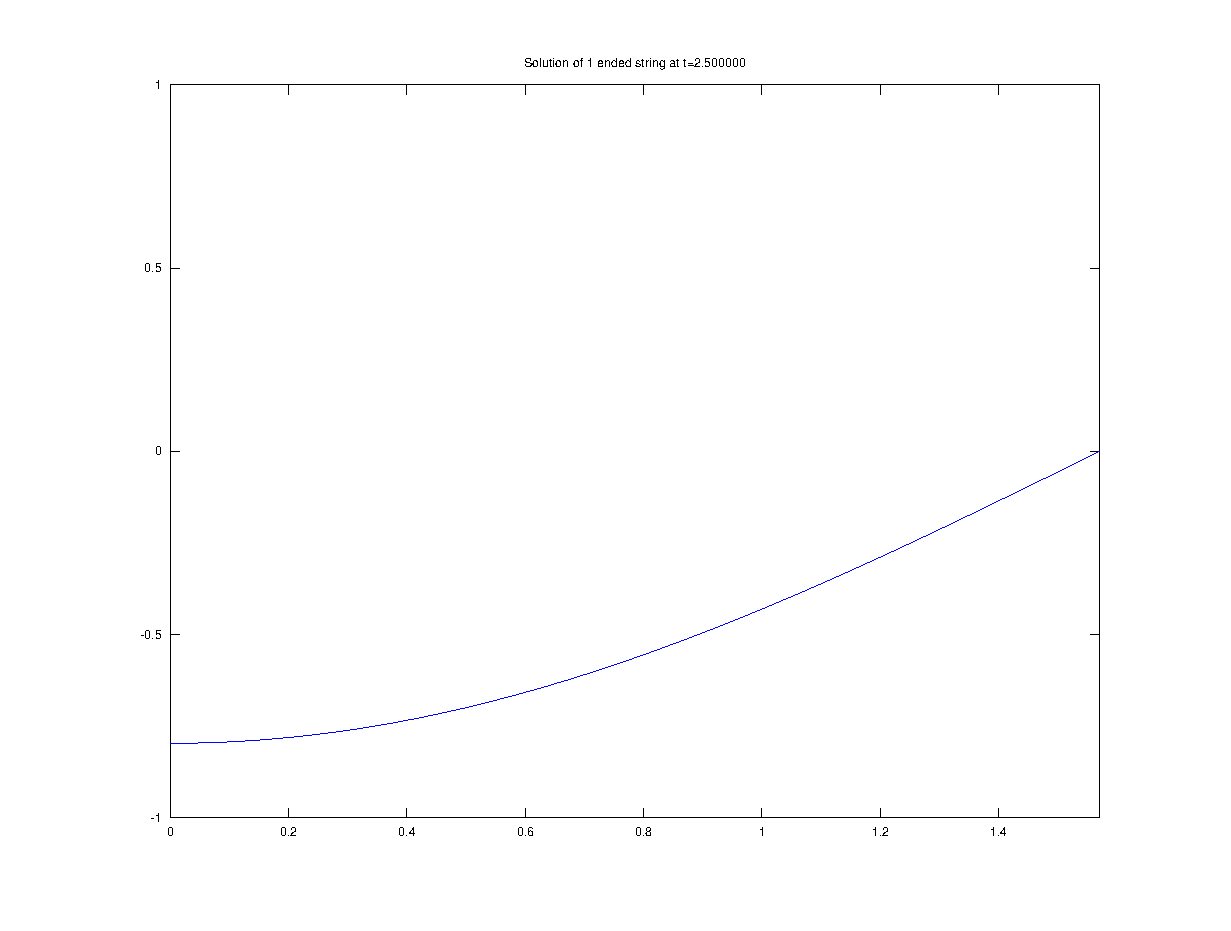
\includegraphics[width=6cm]{./one_fixed_end_analytic_t2.500000.eps}
 % fixed_ends_analytic.eps: 0x0 pixel, 300dpi, 0.00x0.00 cm, bb=
%\end{center}

\caption{Initial value problem, a string fixed on one end, t=2 and 2.5}

\end{figure} 

\begin{figure}
%\begin{center}
 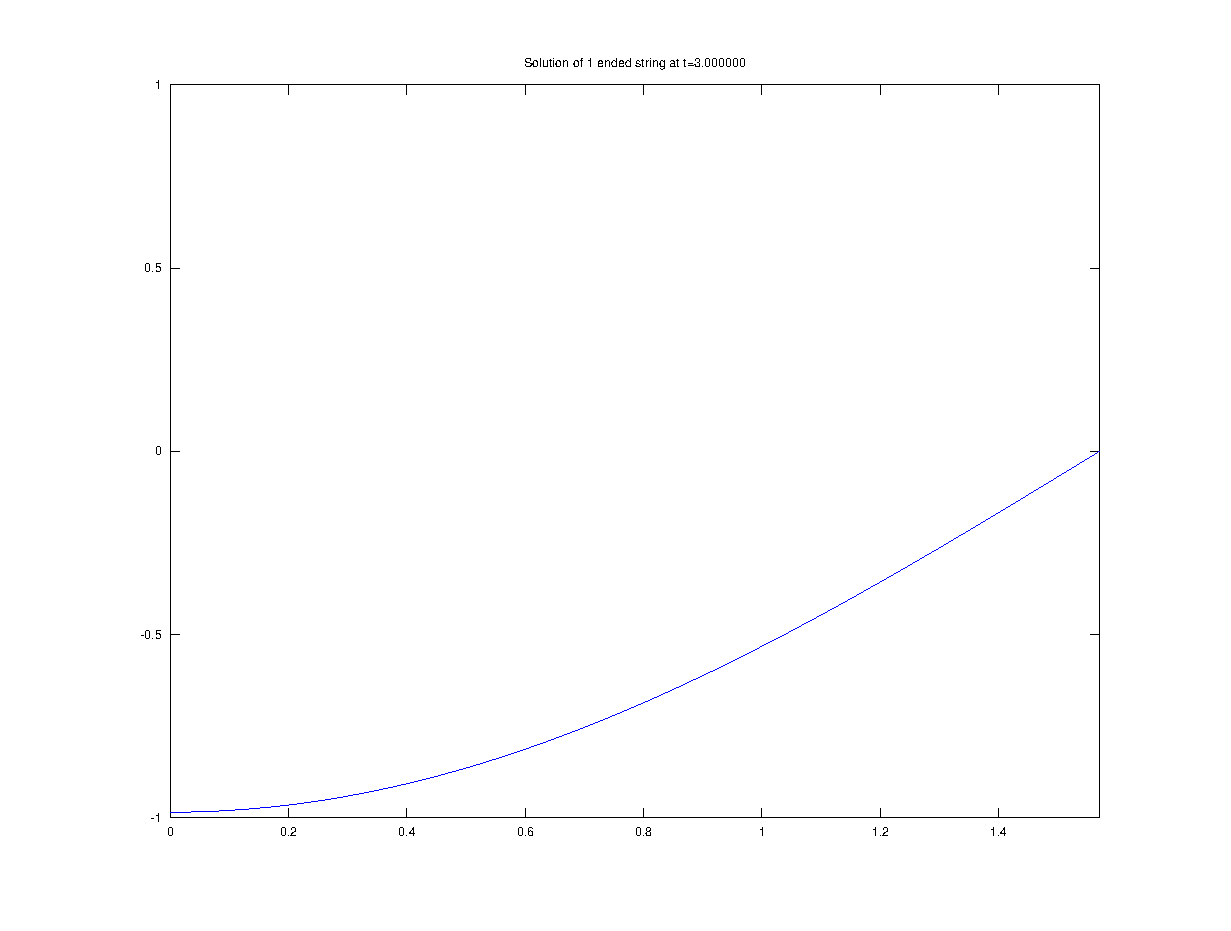
\includegraphics[width=6cm]{./one_fixed_end_analytic_t3.000000.eps}
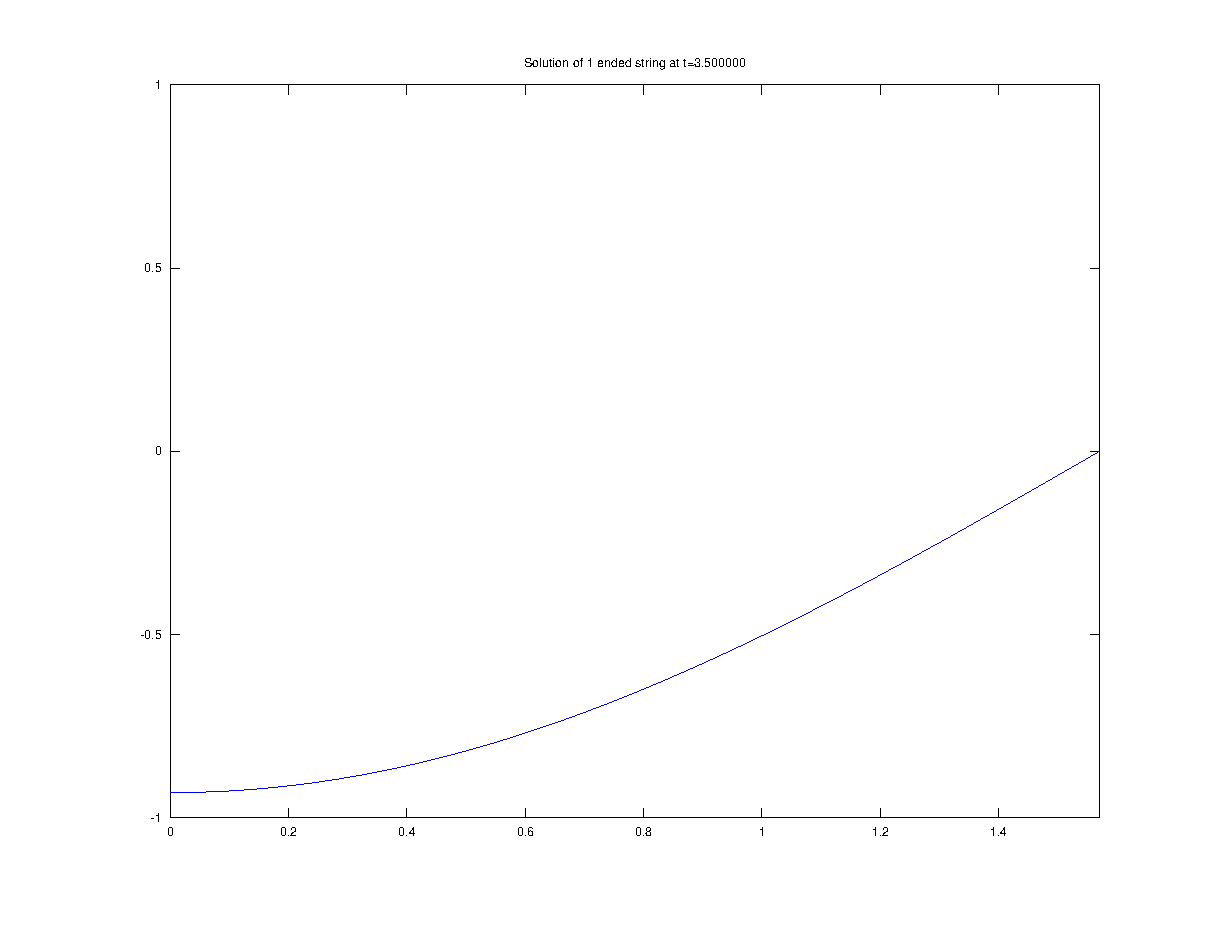
\includegraphics[width=6cm]{./one_fixed_end_analytic_t3.500000.eps}
 % fixed_ends_analytic.eps: 0x0 pixel, 300dpi, 0.00x0.00 cm, bb=
%\end{center}

\caption{Initial value problem, a string fixed on one end, t=3 and 3.5}

\end{figure} 

\begin{figure}
%\begin{center}
 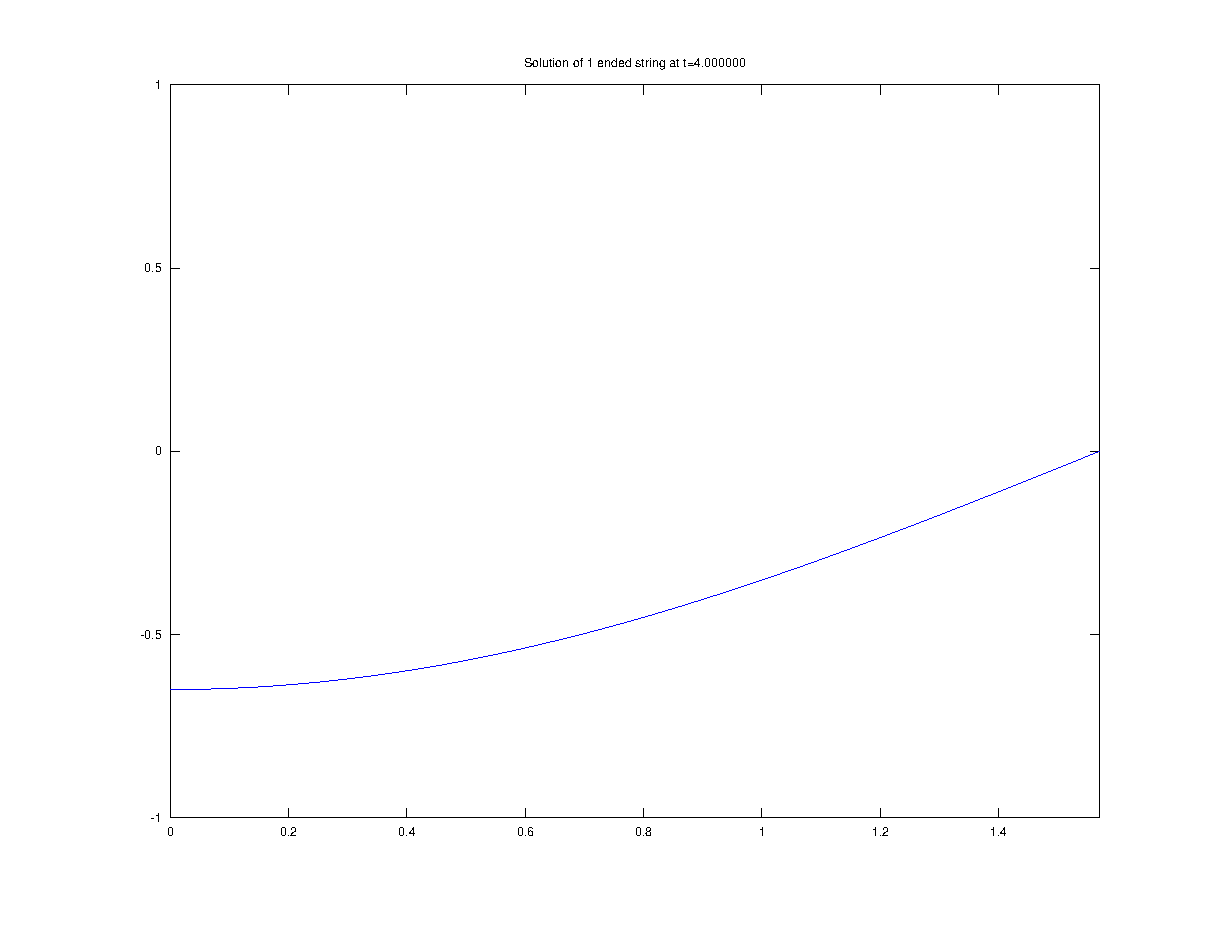
\includegraphics[width=6cm]{./one_fixed_end_analytic_t4.000000.eps}
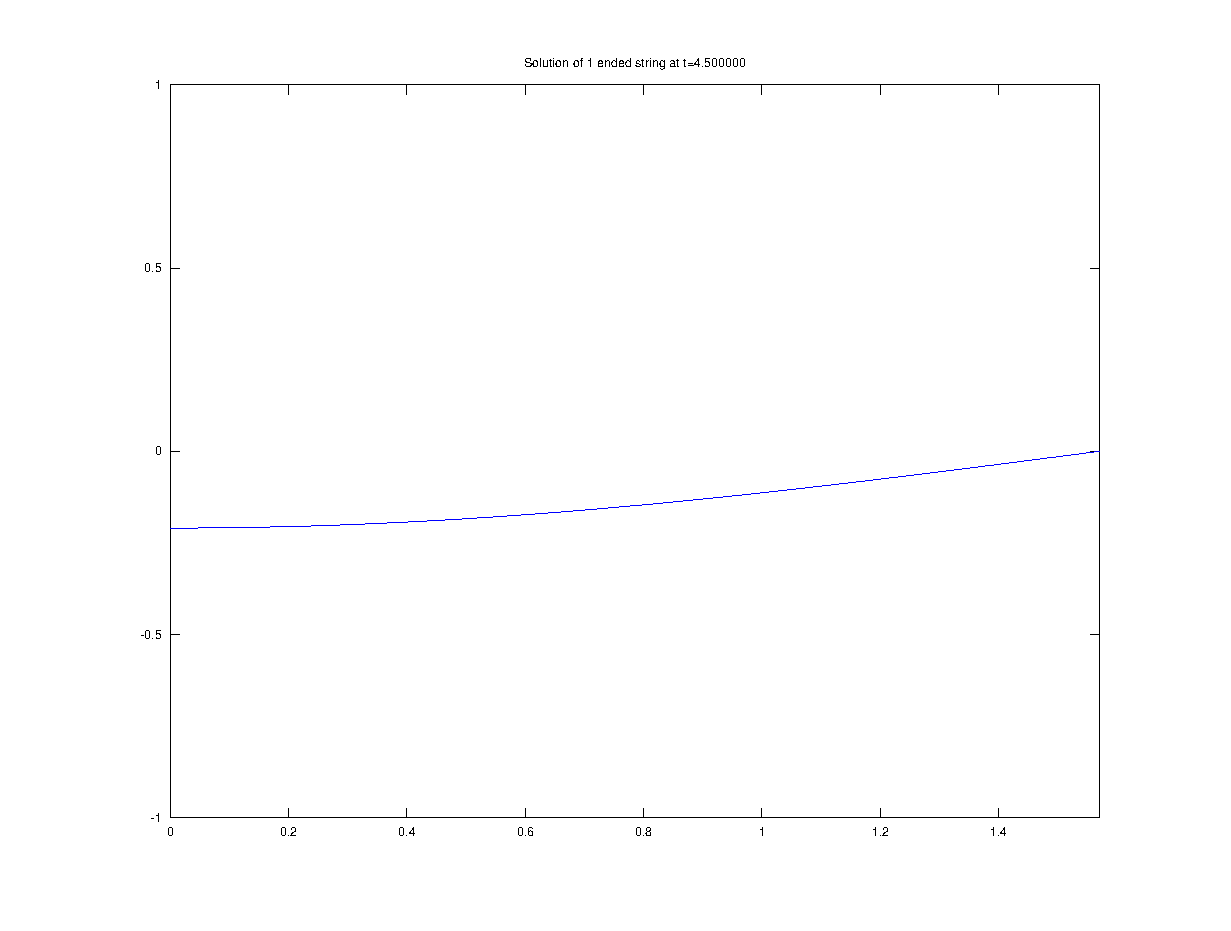
\includegraphics[width=6cm]{./one_fixed_end_analytic_t4.500000.eps}
 % fixed_ends_analytic.eps: 0x0 pixel, 300dpi, 0.00x0.00 cm, bb=
%\end{center}

\caption{Initial value problem, a string fixed on one end, t=4 and 4.5}

\end{figure} 

\begin{figure}
%\begin{center}
 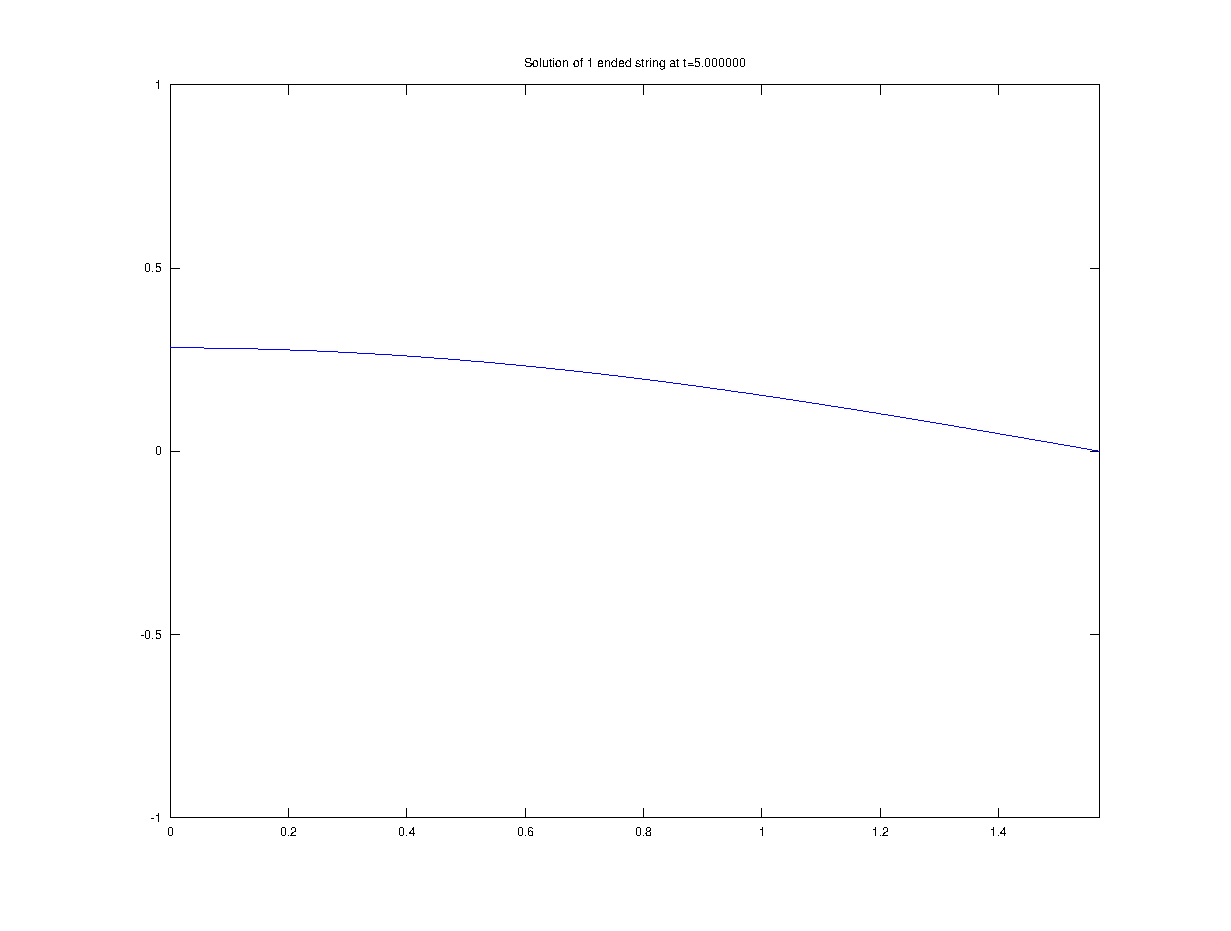
\includegraphics[width=6cm]{./one_fixed_end_analytic_t5.000000.eps}
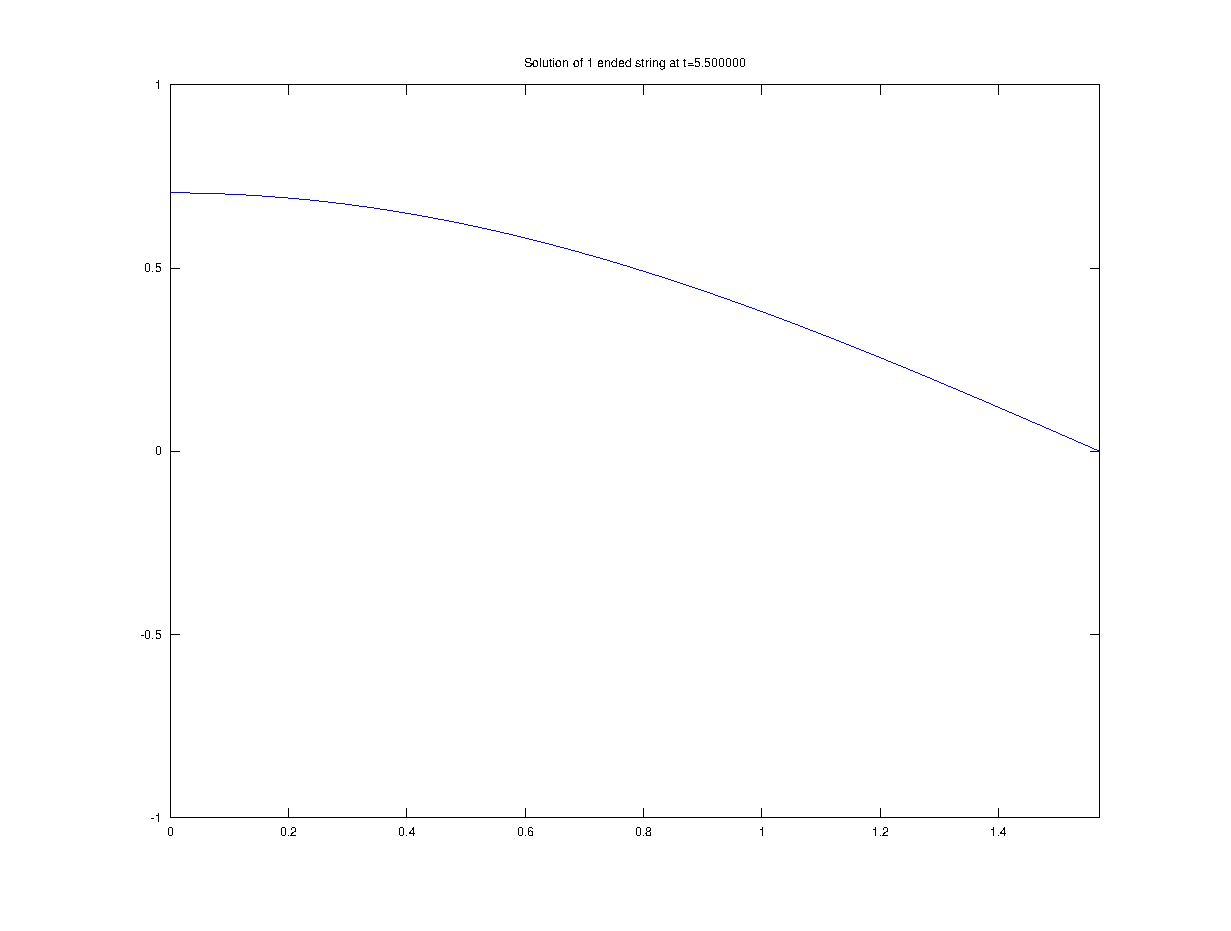
\includegraphics[width=6cm]{./one_fixed_end_analytic_t5.500000.eps}
 % fixed_ends_analytic.eps: 0x0 pixel, 300dpi, 0.00x0.00 cm, bb=
%\end{center}

\caption{Initial value problem, a string fixed on one end, t=5.0 and 5.5}

\end{figure} 

\begin{figure}
%\begin{center}
 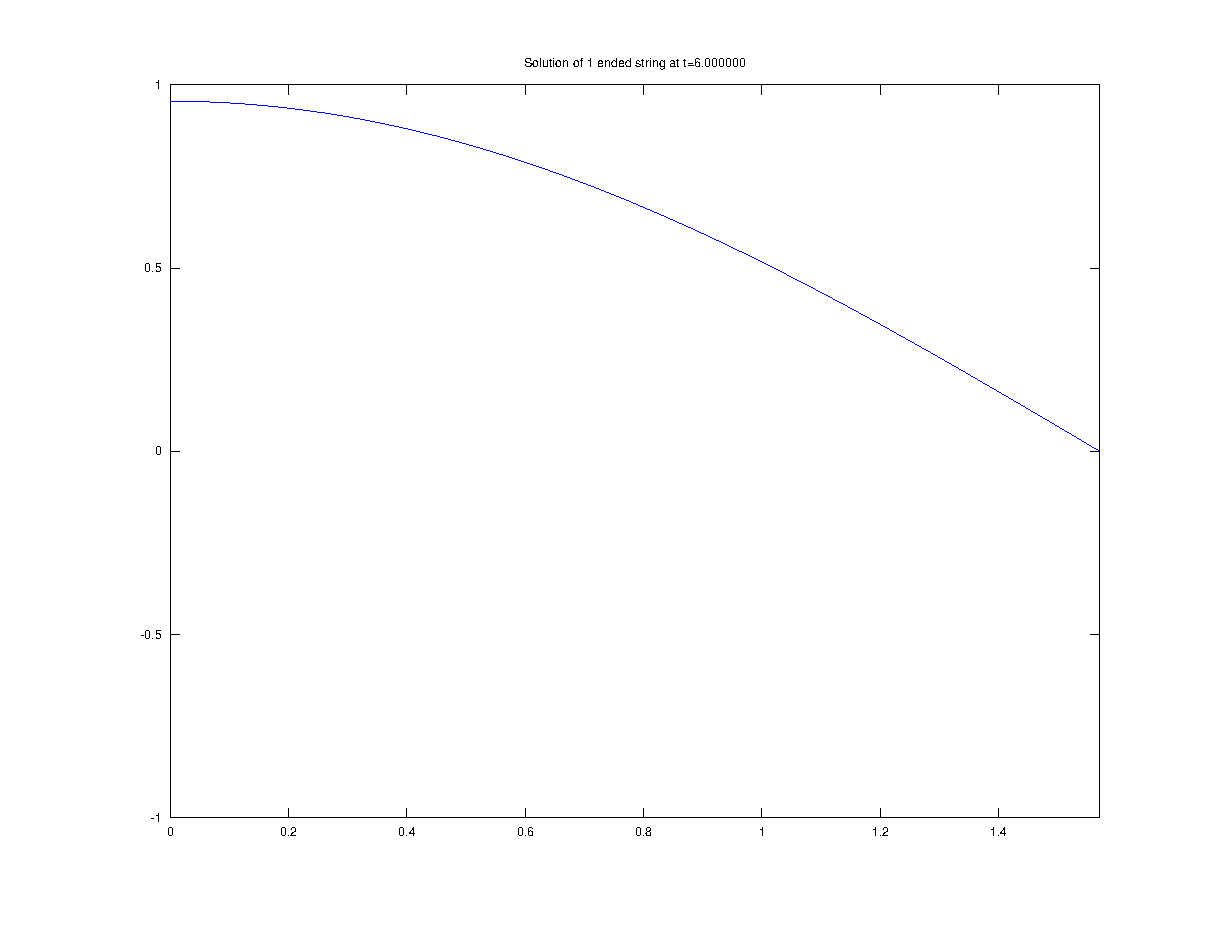
\includegraphics[width=6cm]{./one_fixed_end_analytic_t6.000000.eps}
 % fixed_ends_analytic.eps: 0x0 pixel, 300dpi, 0.00x0.00 cm, bb=
%\end{center}

\caption{Initial value problem, a string fixed on one end, t=6}
\label{fig:half_bounded_2}
\end{figure} 

\end{document}          
